%\section{Characterisation of the electron control regions}
%\label{sec:yields}
%
%The event selection criteria defining the electron control regions are
%detailed in Sec.~\ref{sec:selection}. A selection of relevant data/MC
%comparison plots are presented here. The distributions are shown
%separetely according three \njet categories: symmetric, asymmetric,
%and monojet. The distributions are intended to provide a qualitative
%understanding of the simulation modelling for key variables. However,
%the analysis is not sensitive due the reliance on simulation via
%ratios only (\ie transfer factors) and the one-to-one mapping of
%(\njet,~\nb,~\scalht) binning between the control and signal
%regions. The simulated distributions are normalized to an integrated
%luminosity of 1280.2~$\ifb$ (the data/MC scale factors are also shown
%in all plots).
%
%%The yields in the \mj, \mmj, \ej, \eej and \gj control samples can be
%%found in Tables~\ref{tab:yields_ewk_mu}, \ref{tab:yields_ewk_mumu},
%%and \ref{tab:yields_ewk_gj} respectively for 1.28 \ifb (yields for
%%3\ifb are in Appendix~\ref{app:yields3fb}).  The number of events in
%%each of these regions is important to determine how these analysis
%%regions can be extended. We require to each control region to have
%%sufficiently populated control regions to enable a robust data driven
%%background prediction.
%
%\subsection{Yields and distributions for the electron + jets control sample}
%
%\begin{figure}
%    \begin{center}
%        \subfigure {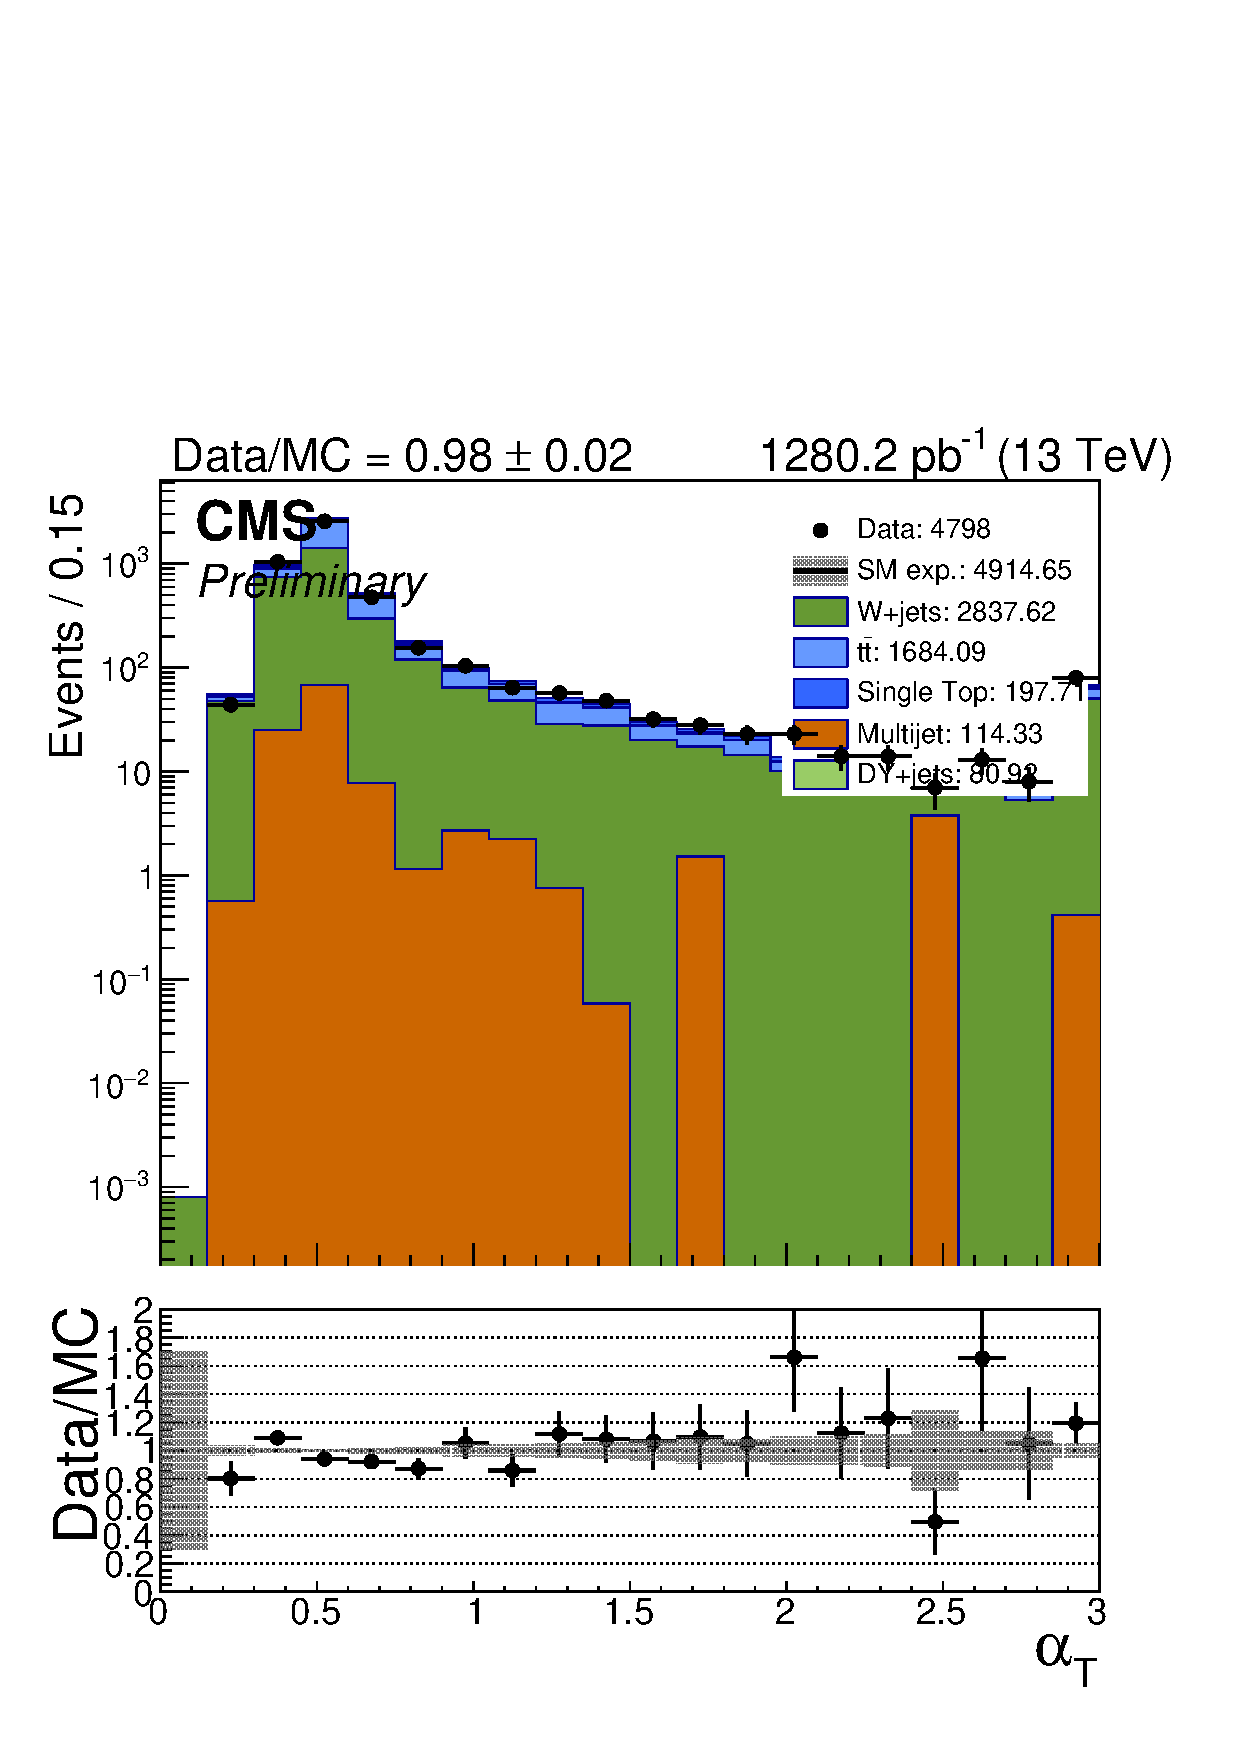
\includegraphics[width=0.5\textwidth]{figures/distributions/SingleEle/alphaT_sym.pdf}} ~~
%        \subfigure {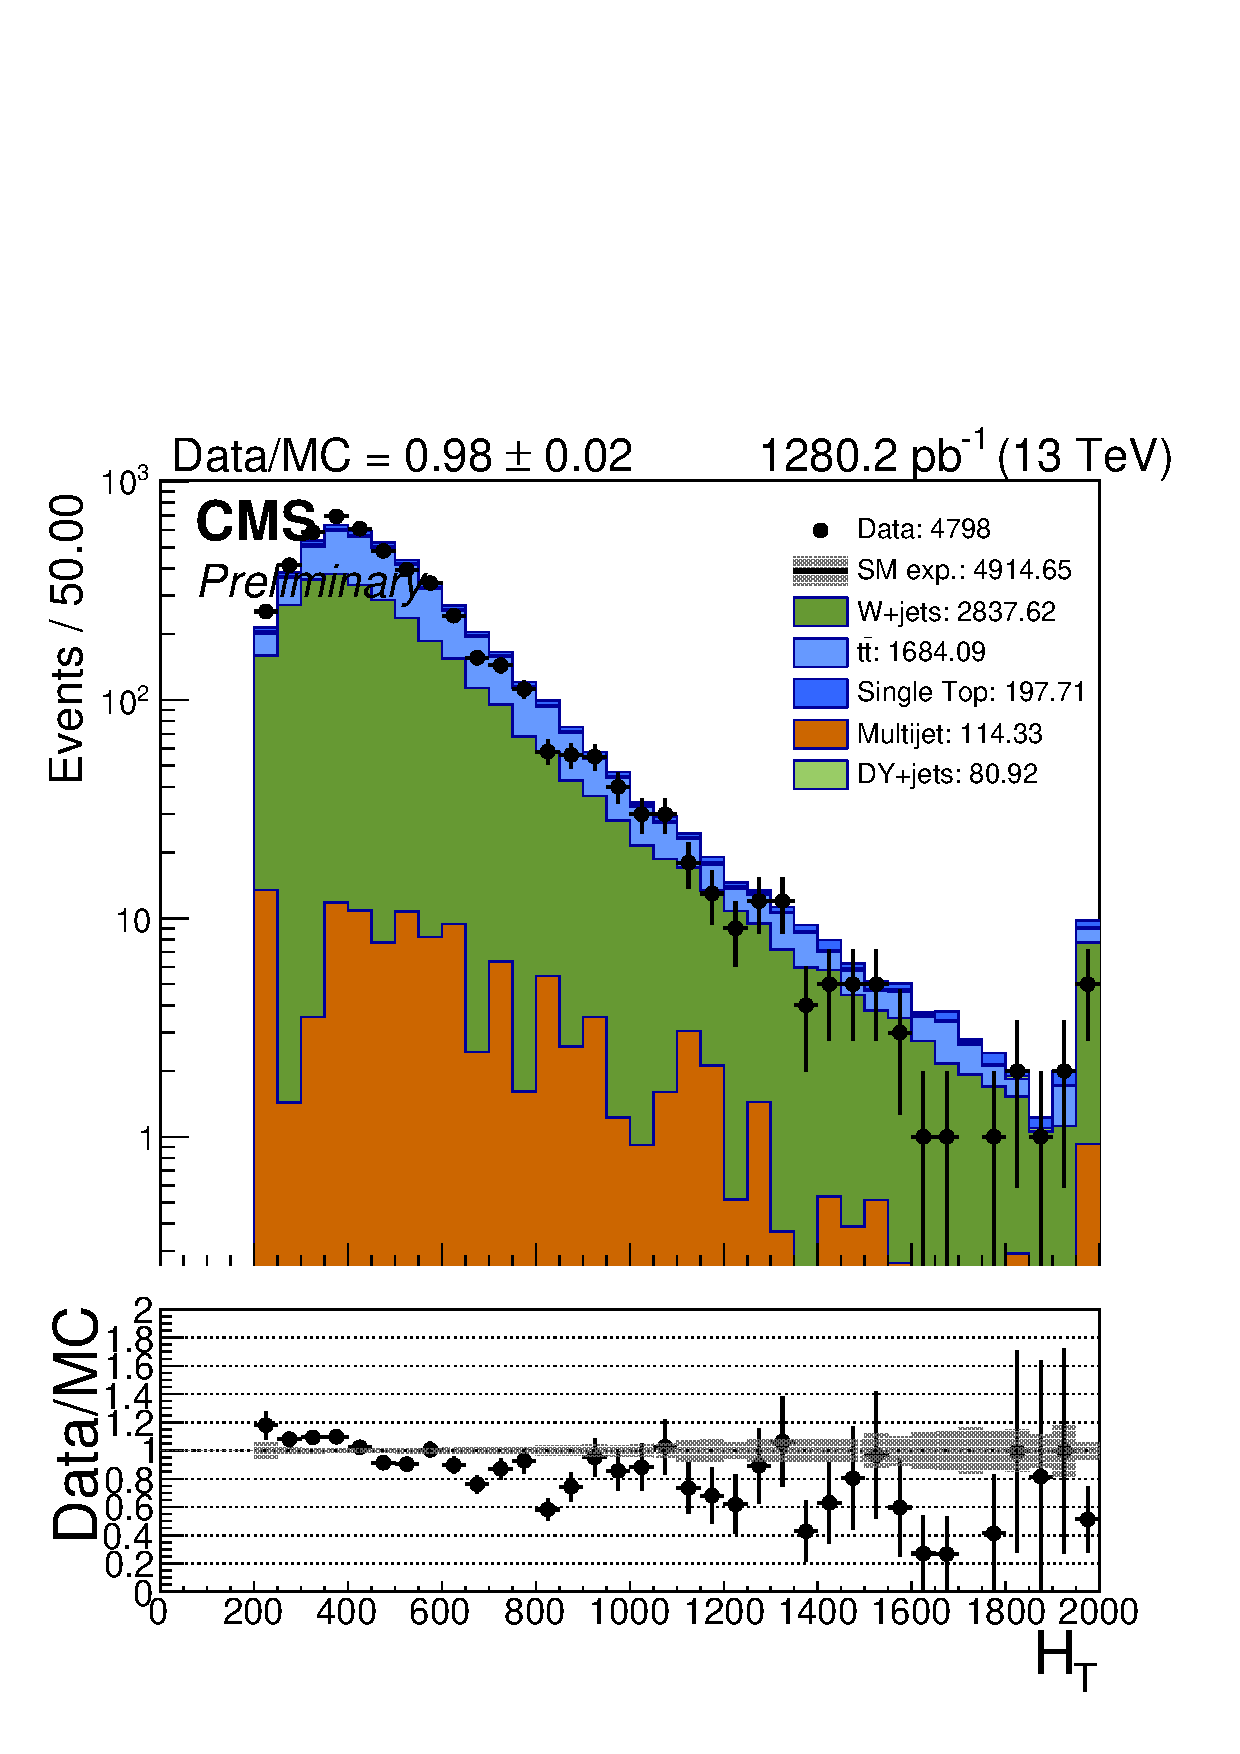
\includegraphics[width=0.5\textwidth]{figures/distributions/SingleEle/ht40_sym.pdf}} \\
%        \subfigure {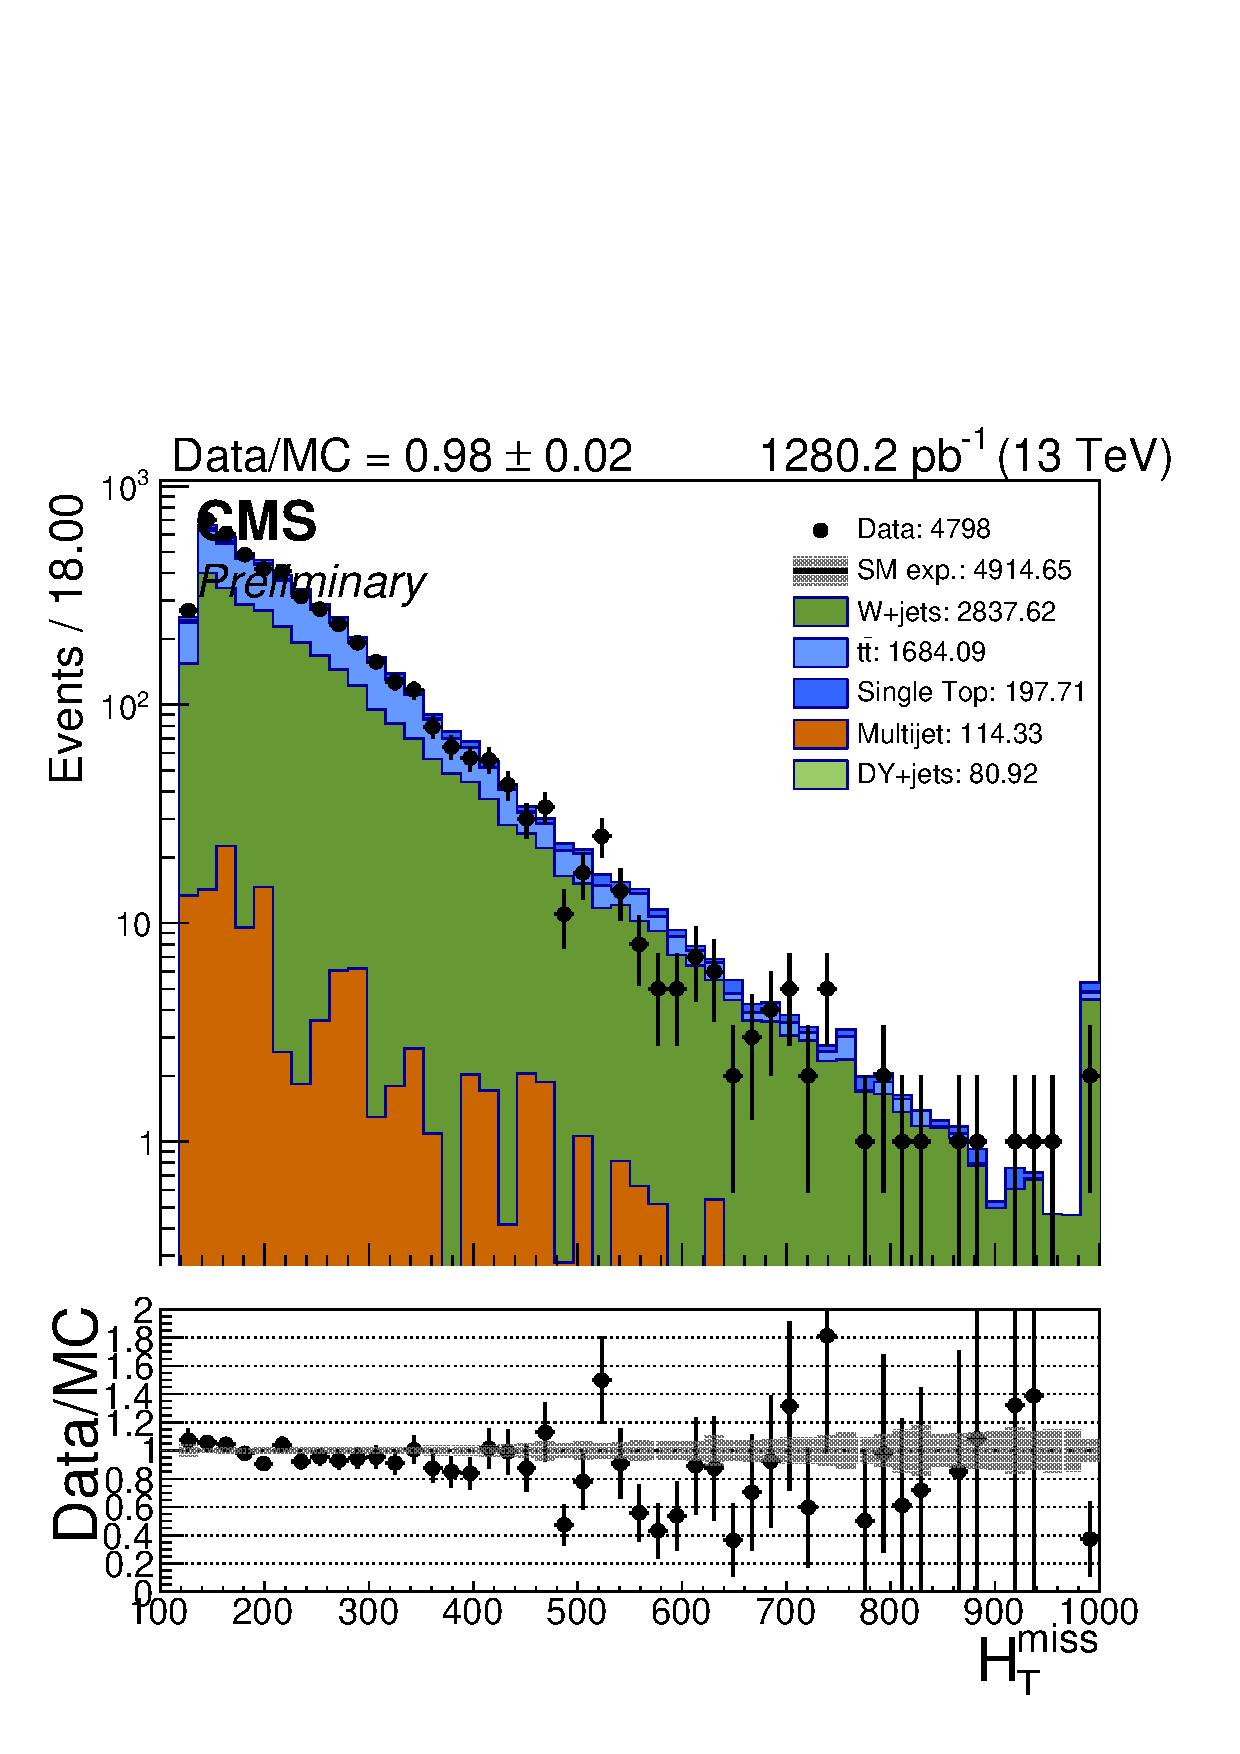
\includegraphics[width=0.5\textwidth]{figures/distributions/SingleEle/mht40_pt_sym.pdf}} ~~
%        \subfigure {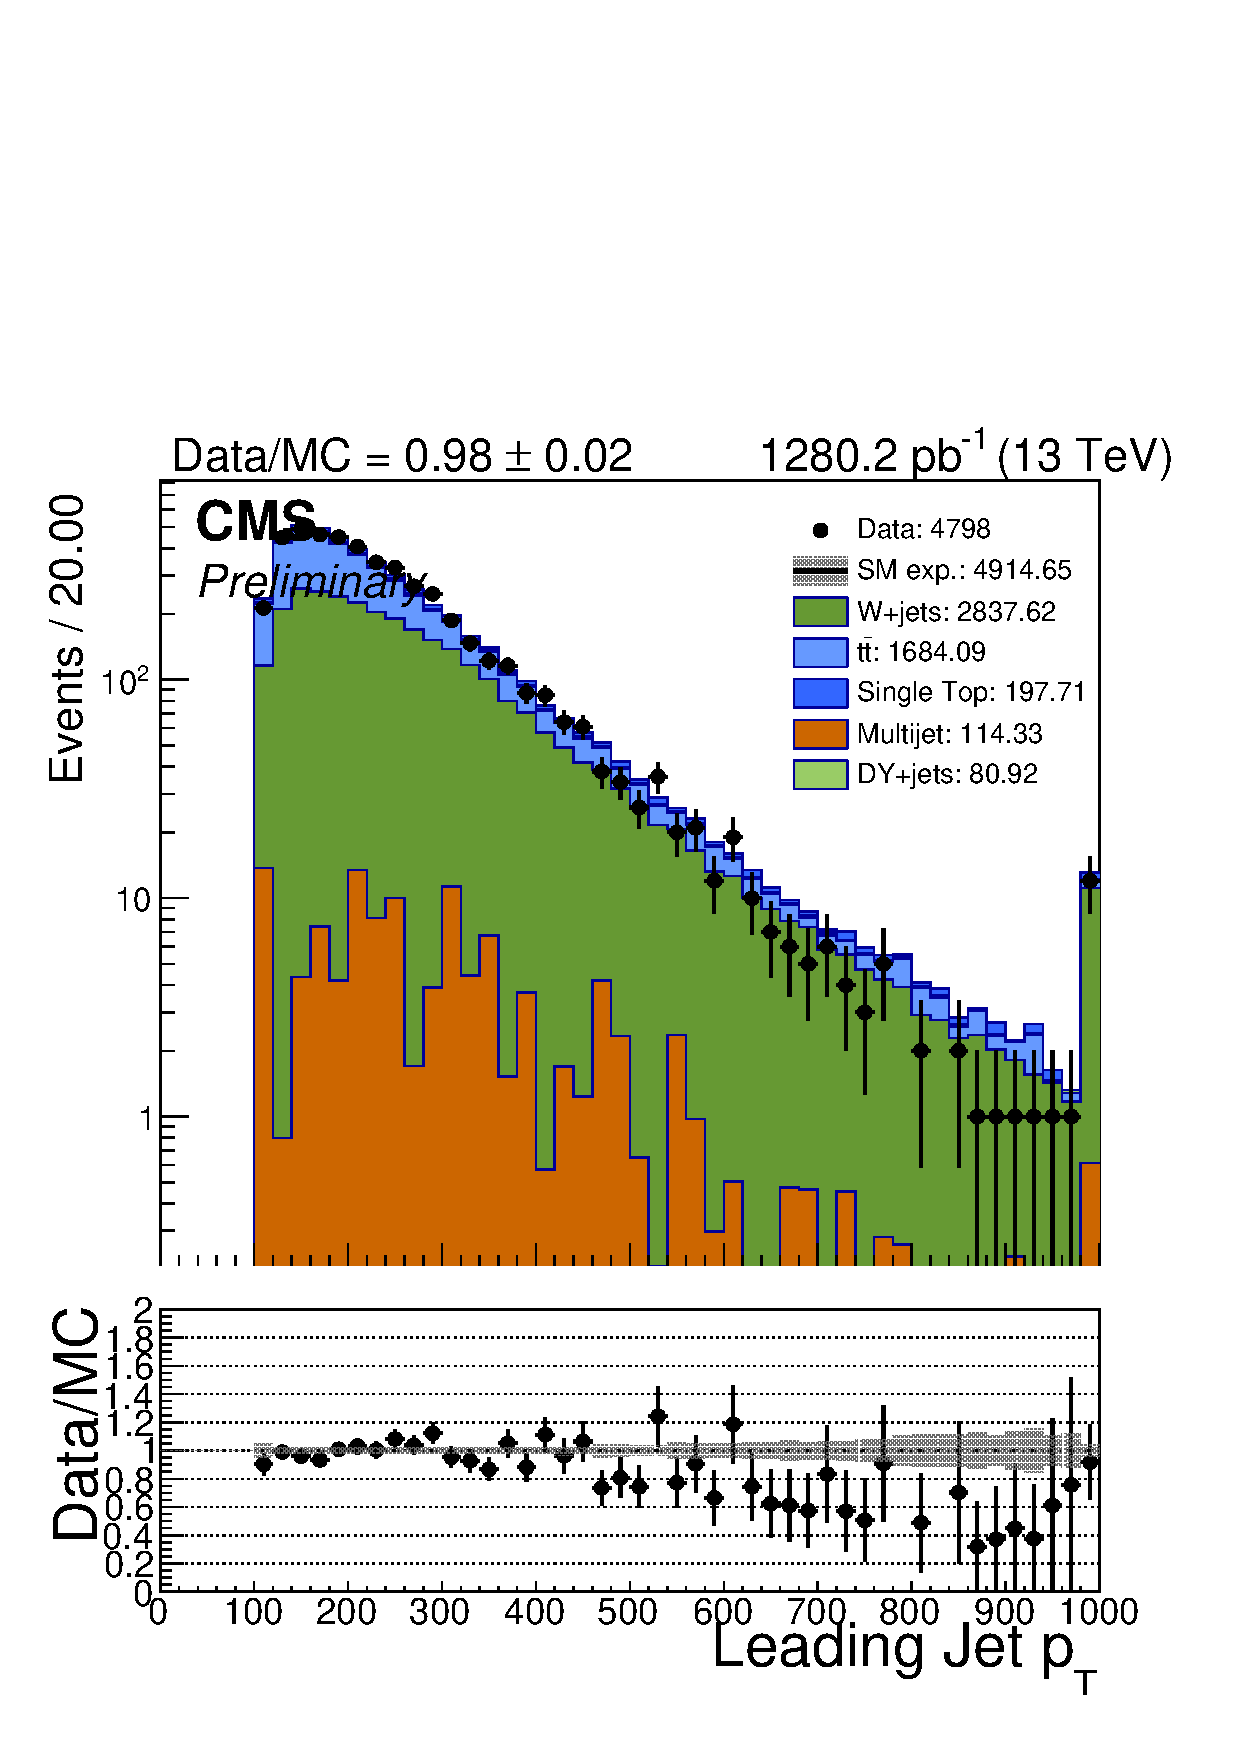
\includegraphics[width=0.5\textwidth]{figures/distributions/SingleEle/jet_pt[0]_sym.pdf}} \\
%        \caption{Key analysis variables for single electron control region (symmetric \njet bins)}
%        \label{fig:distribution_singleele_sym}
%    \end{center}
%\end{figure}
%
%\begin{figure}
%    \begin{center}
%        \subfigure {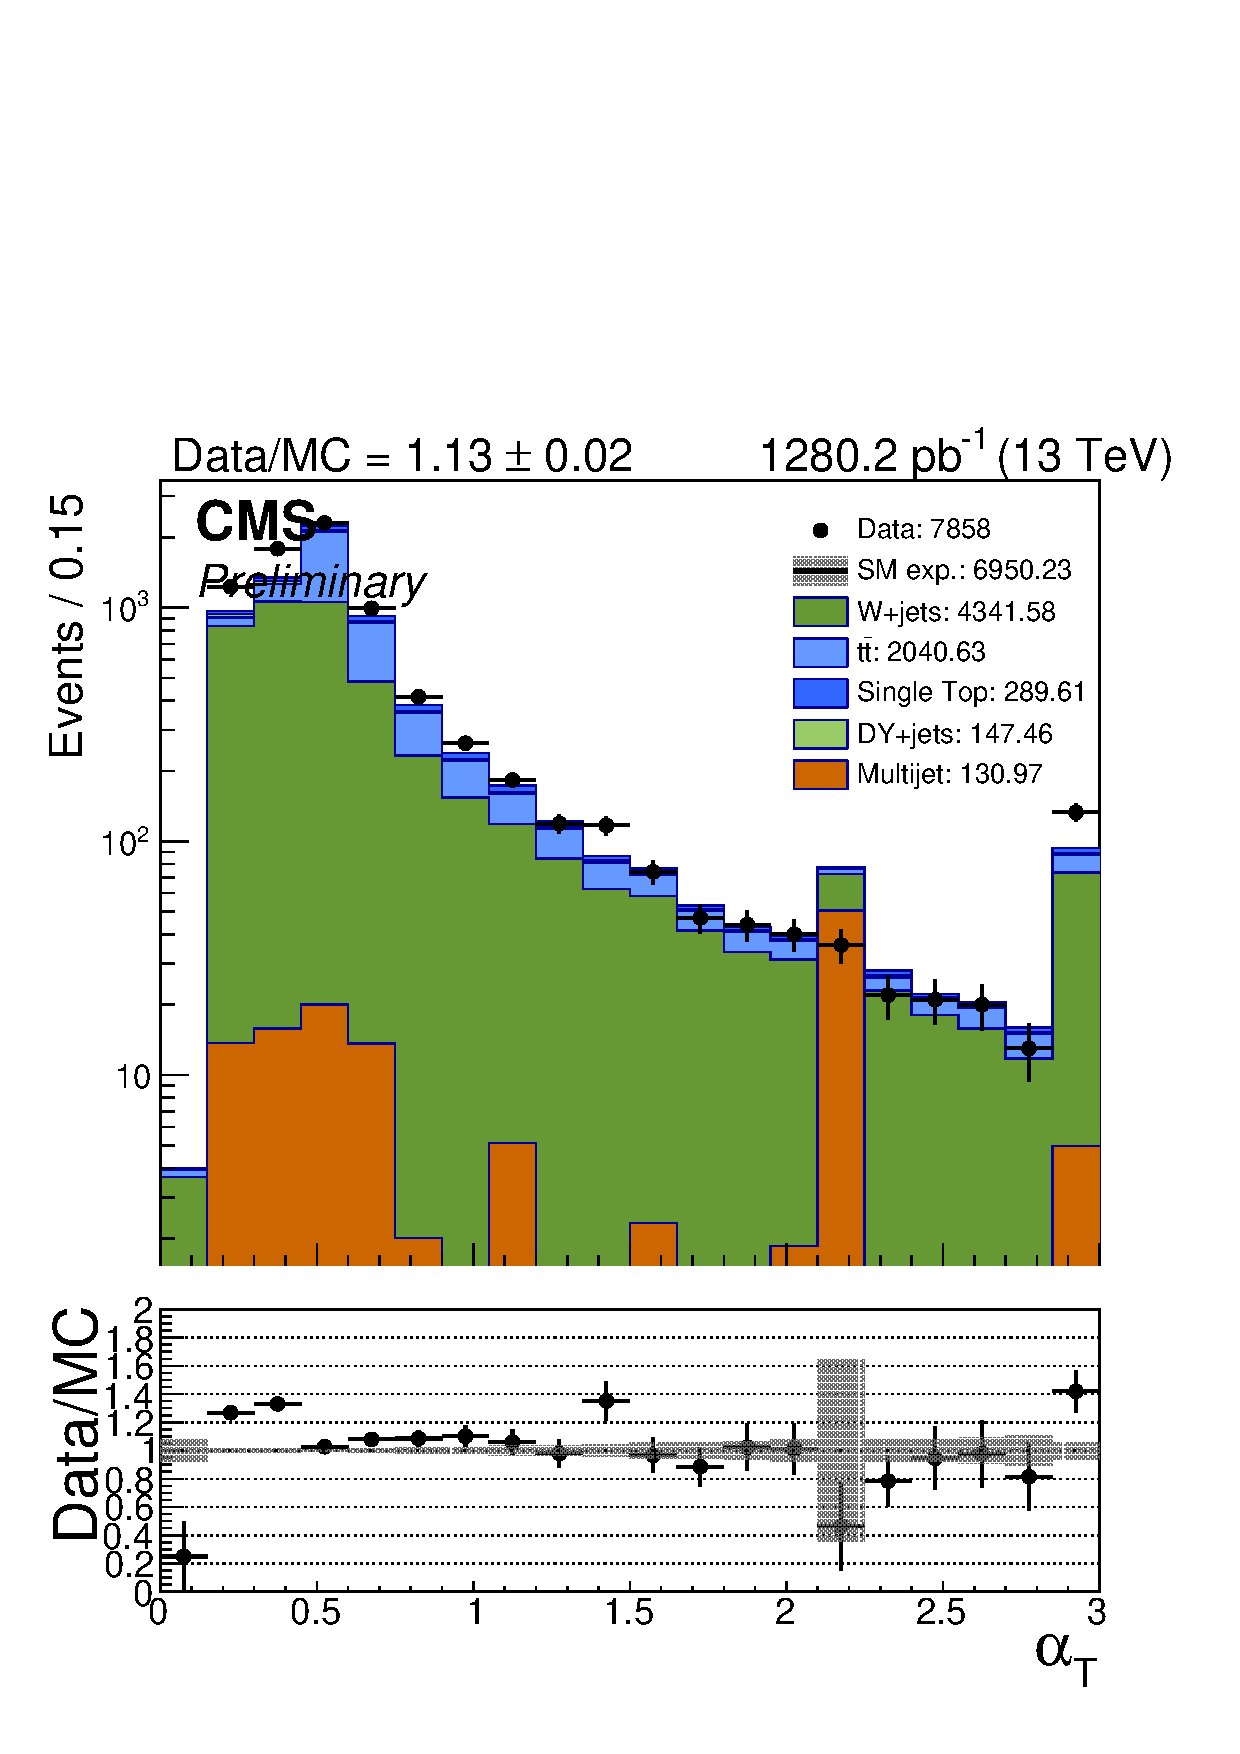
\includegraphics[width=0.5\textwidth]{figures/distributions/SingleEle/alphaT_asym.pdf}} ~~
%        \subfigure {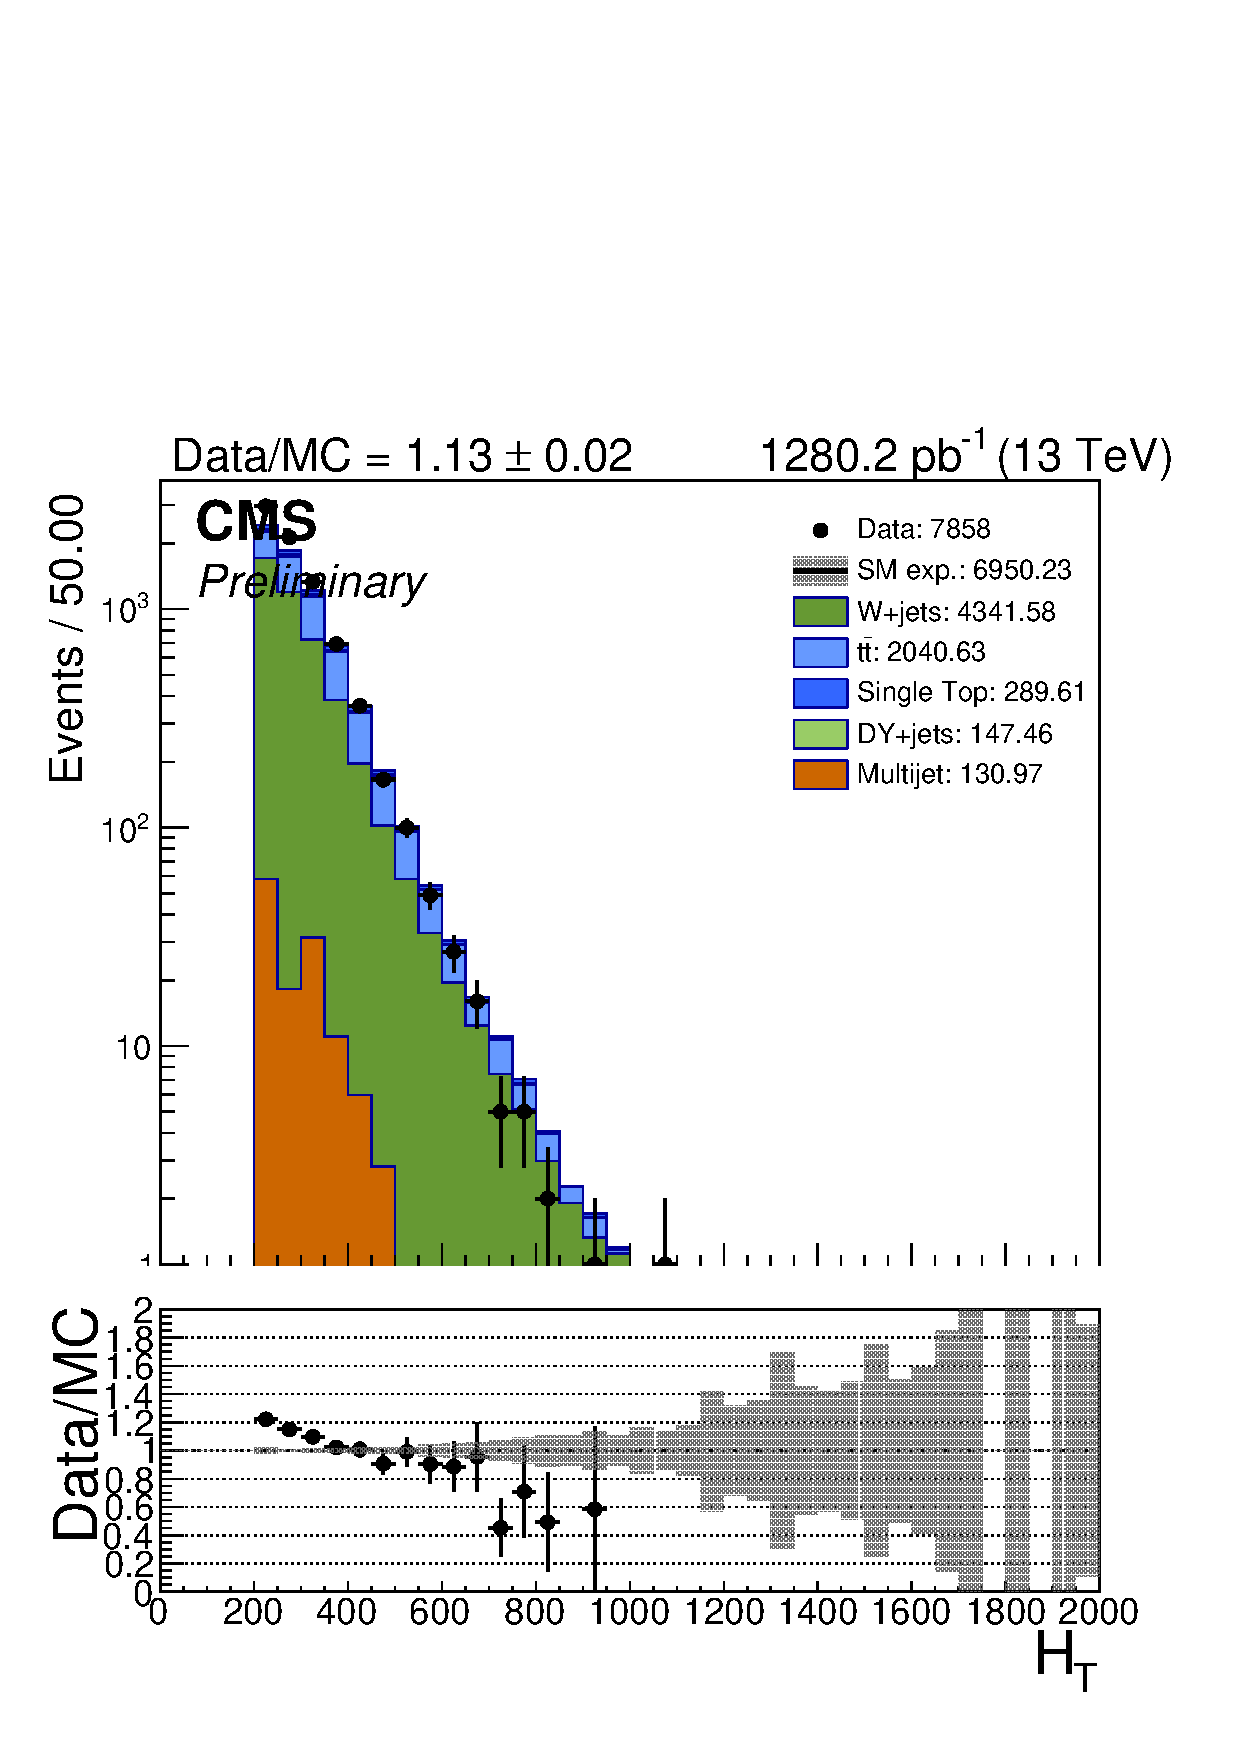
\includegraphics[width=0.5\textwidth]{figures/distributions/SingleEle/ht40_asym.pdf}} \\
%        \subfigure {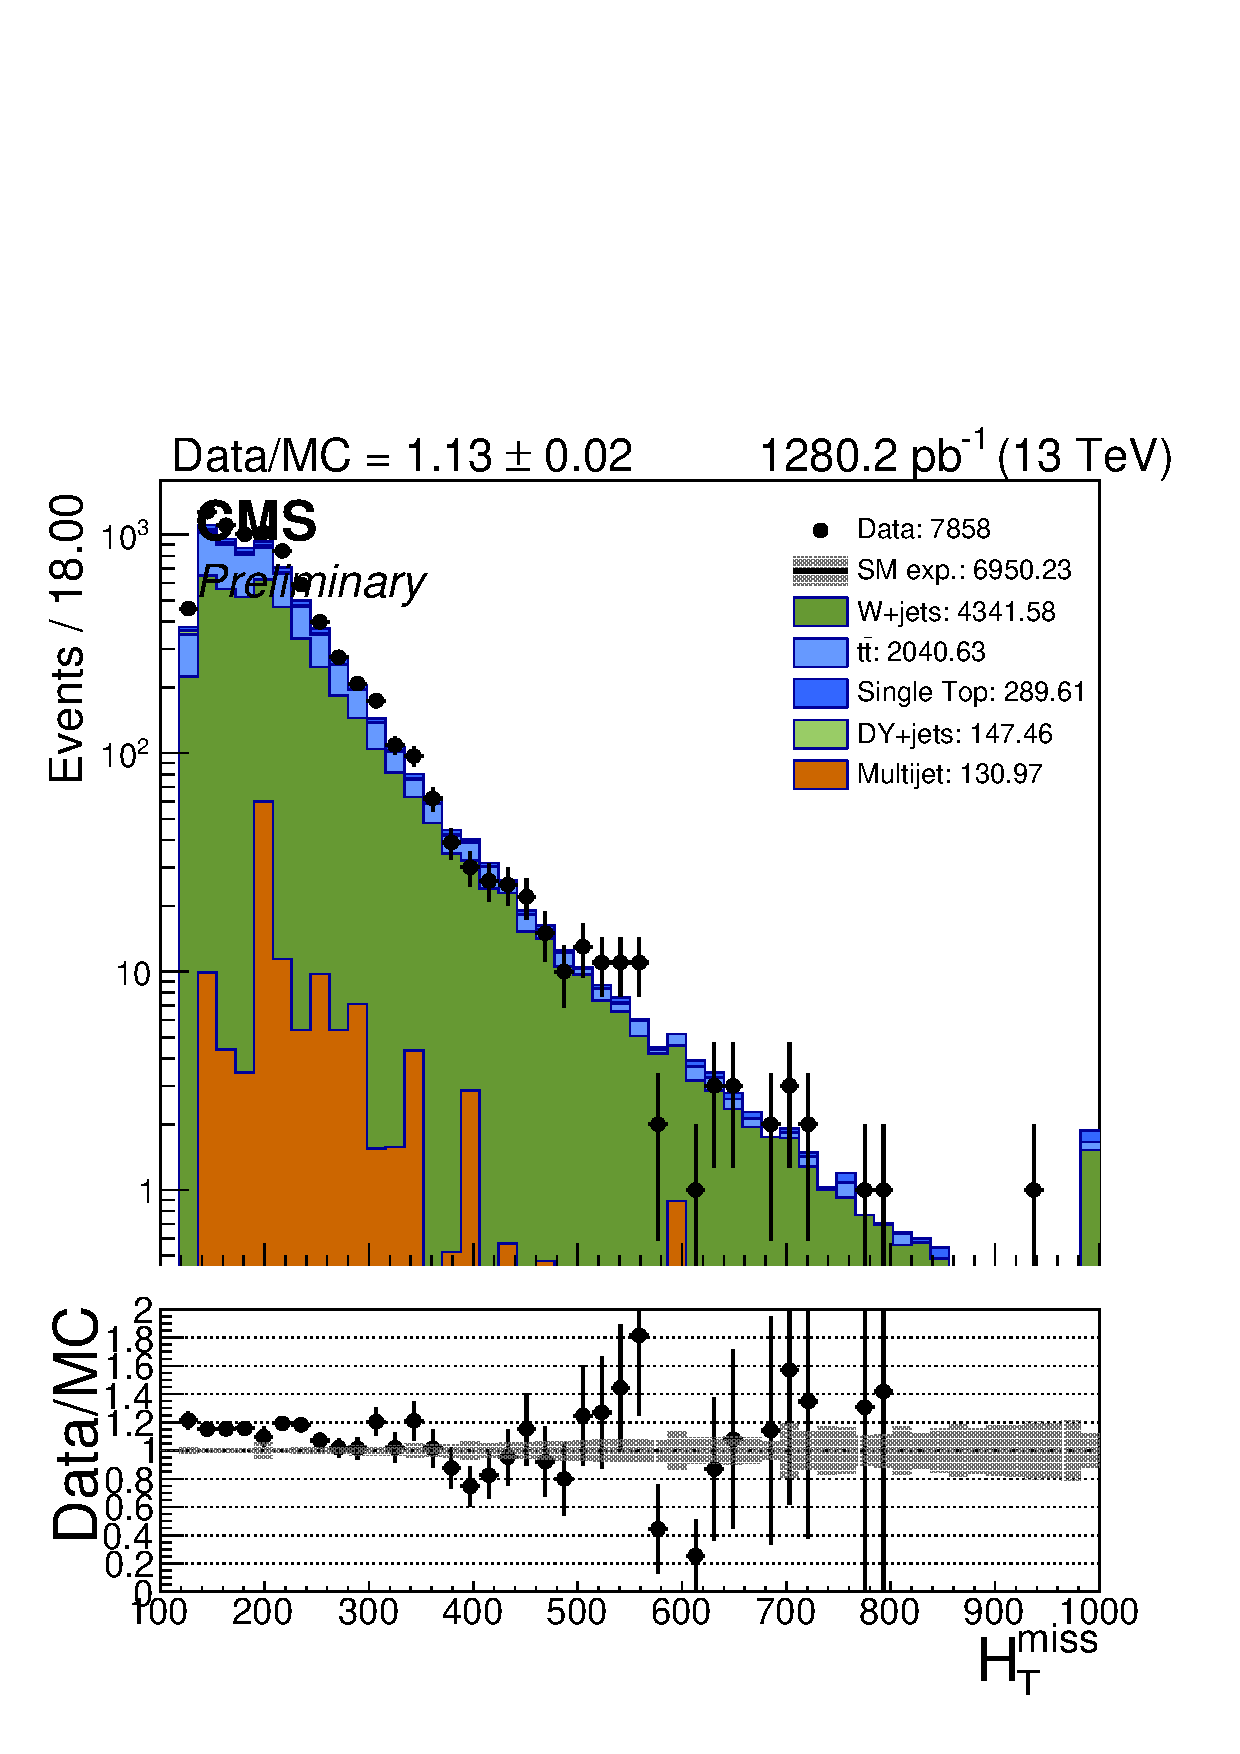
\includegraphics[width=0.5\textwidth]{figures/distributions/SingleEle/mht40_pt_asym.pdf}} ~~
%        \subfigure {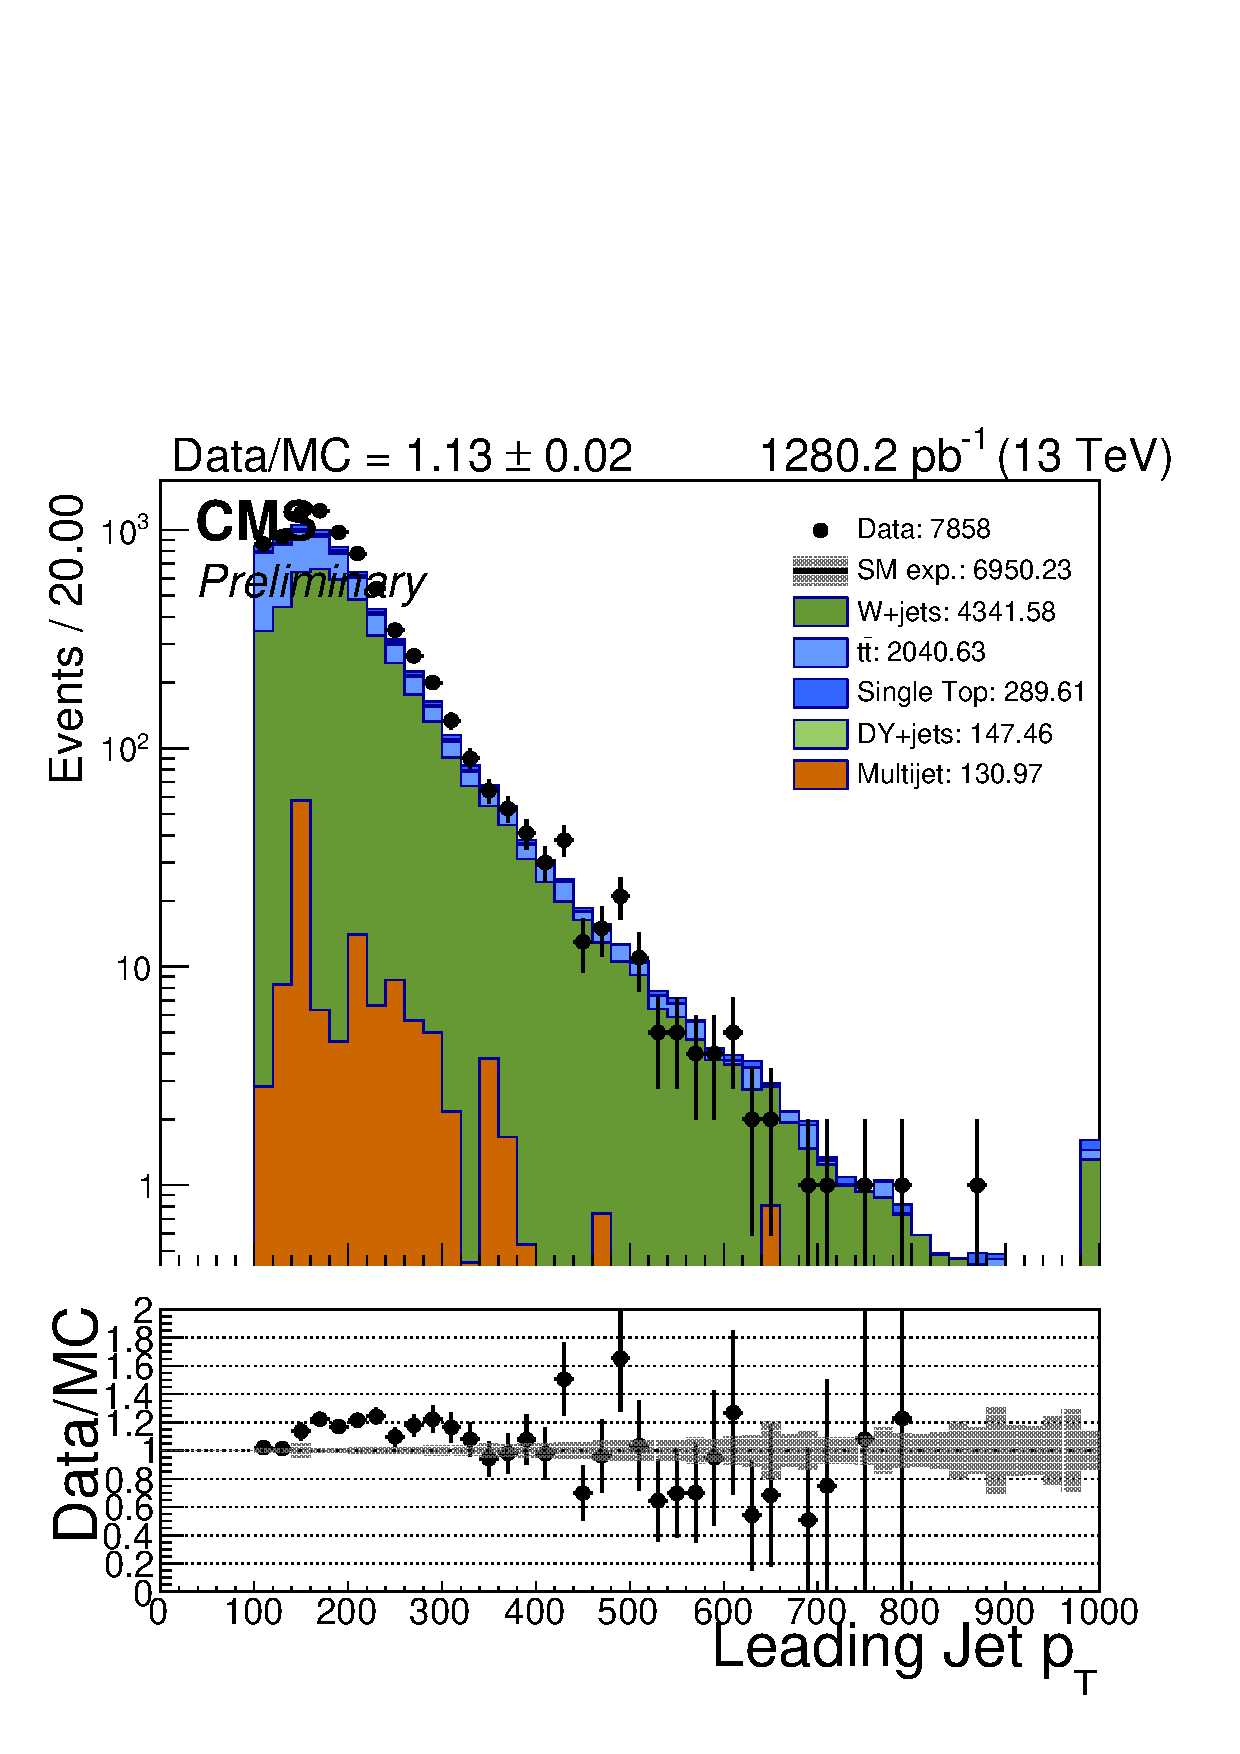
\includegraphics[width=0.5\textwidth]{figures/distributions/SingleEle/jet_pt[0]_asym.pdf}} \\
%        \caption{Key analysis variables for single electron control region (asymmetric \njet bins)}
%        \label{fig:distribution_singleele_asym}
%    \end{center}
%\end{figure}
%
%\begin{figure}
%    \begin{center} 
%        \subfigure {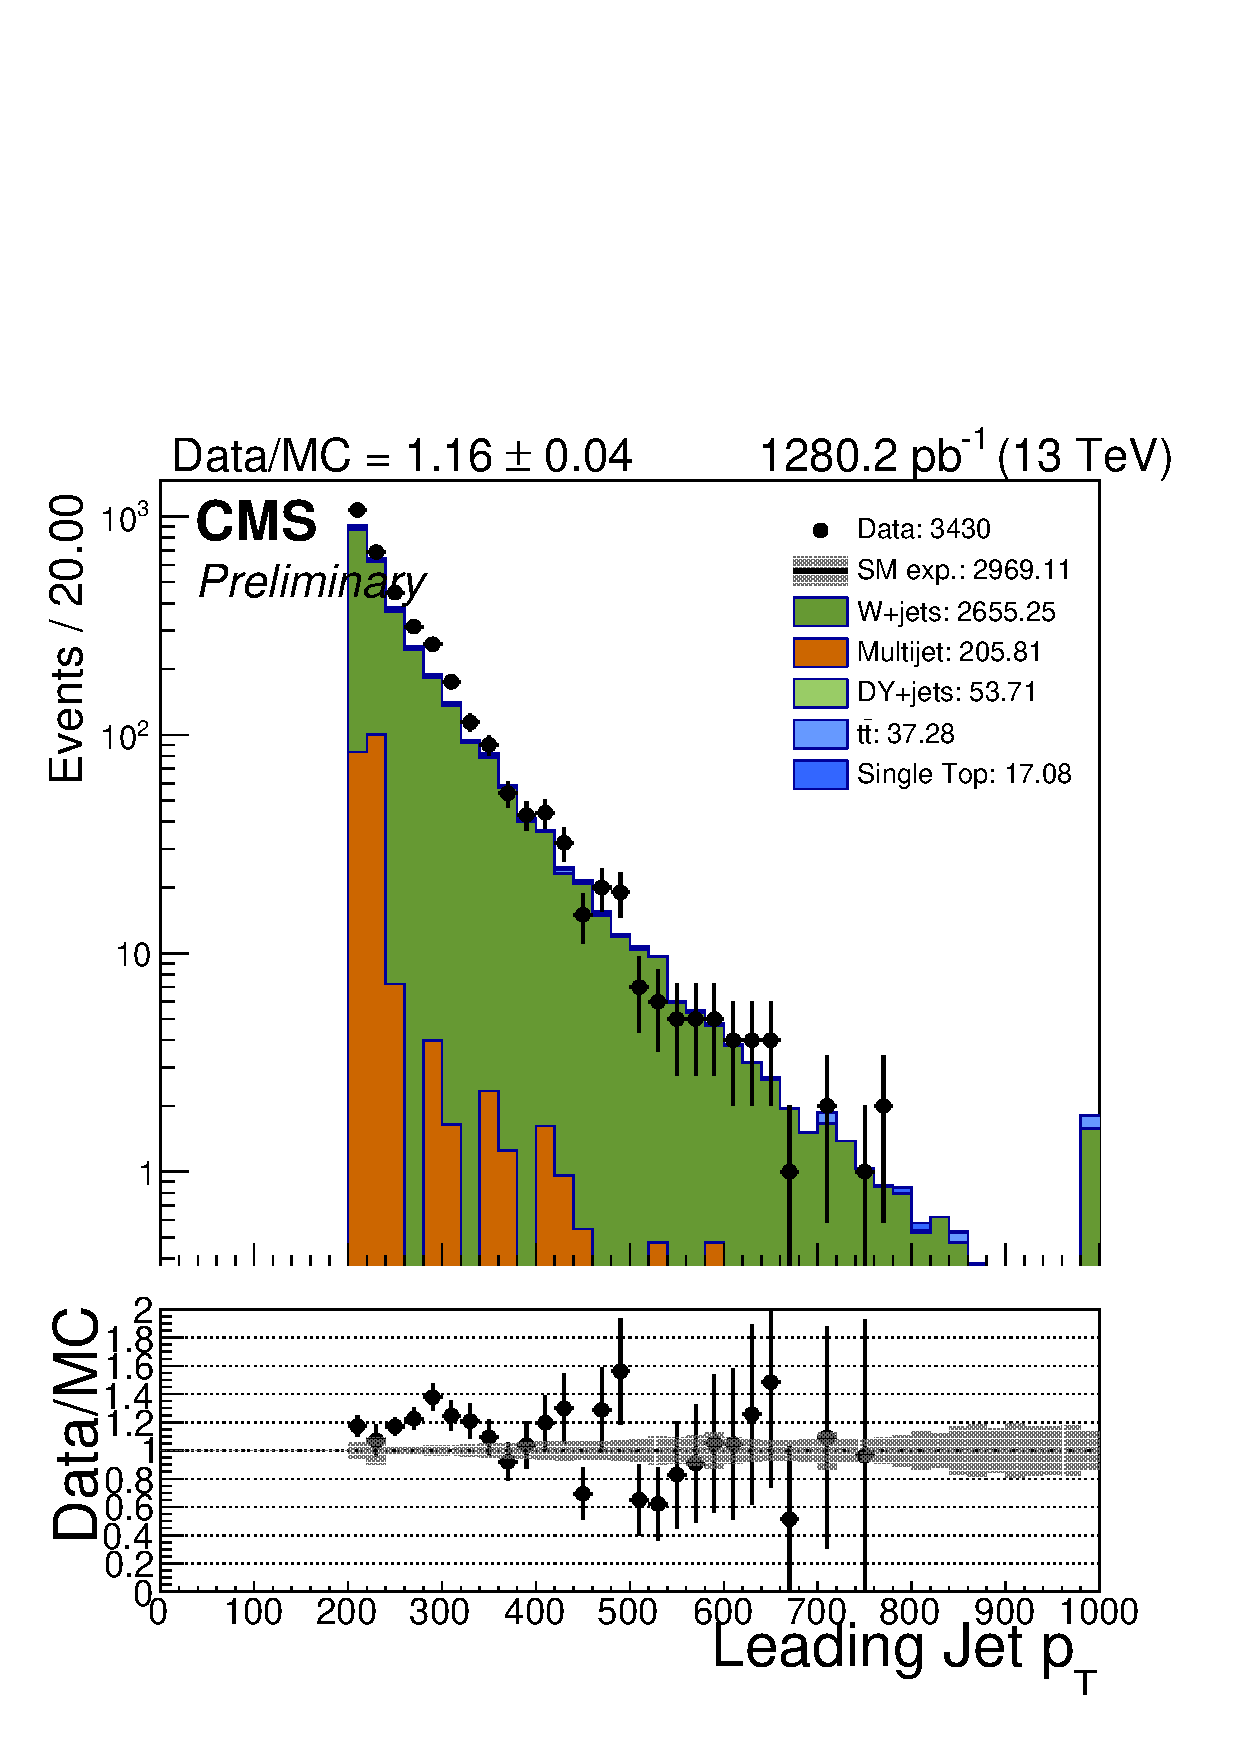
\includegraphics[width=0.5\textwidth]{figures/distributions/SingleEle/jet_pt[0]_eq1j.pdf}} ~~
%        \subfigure {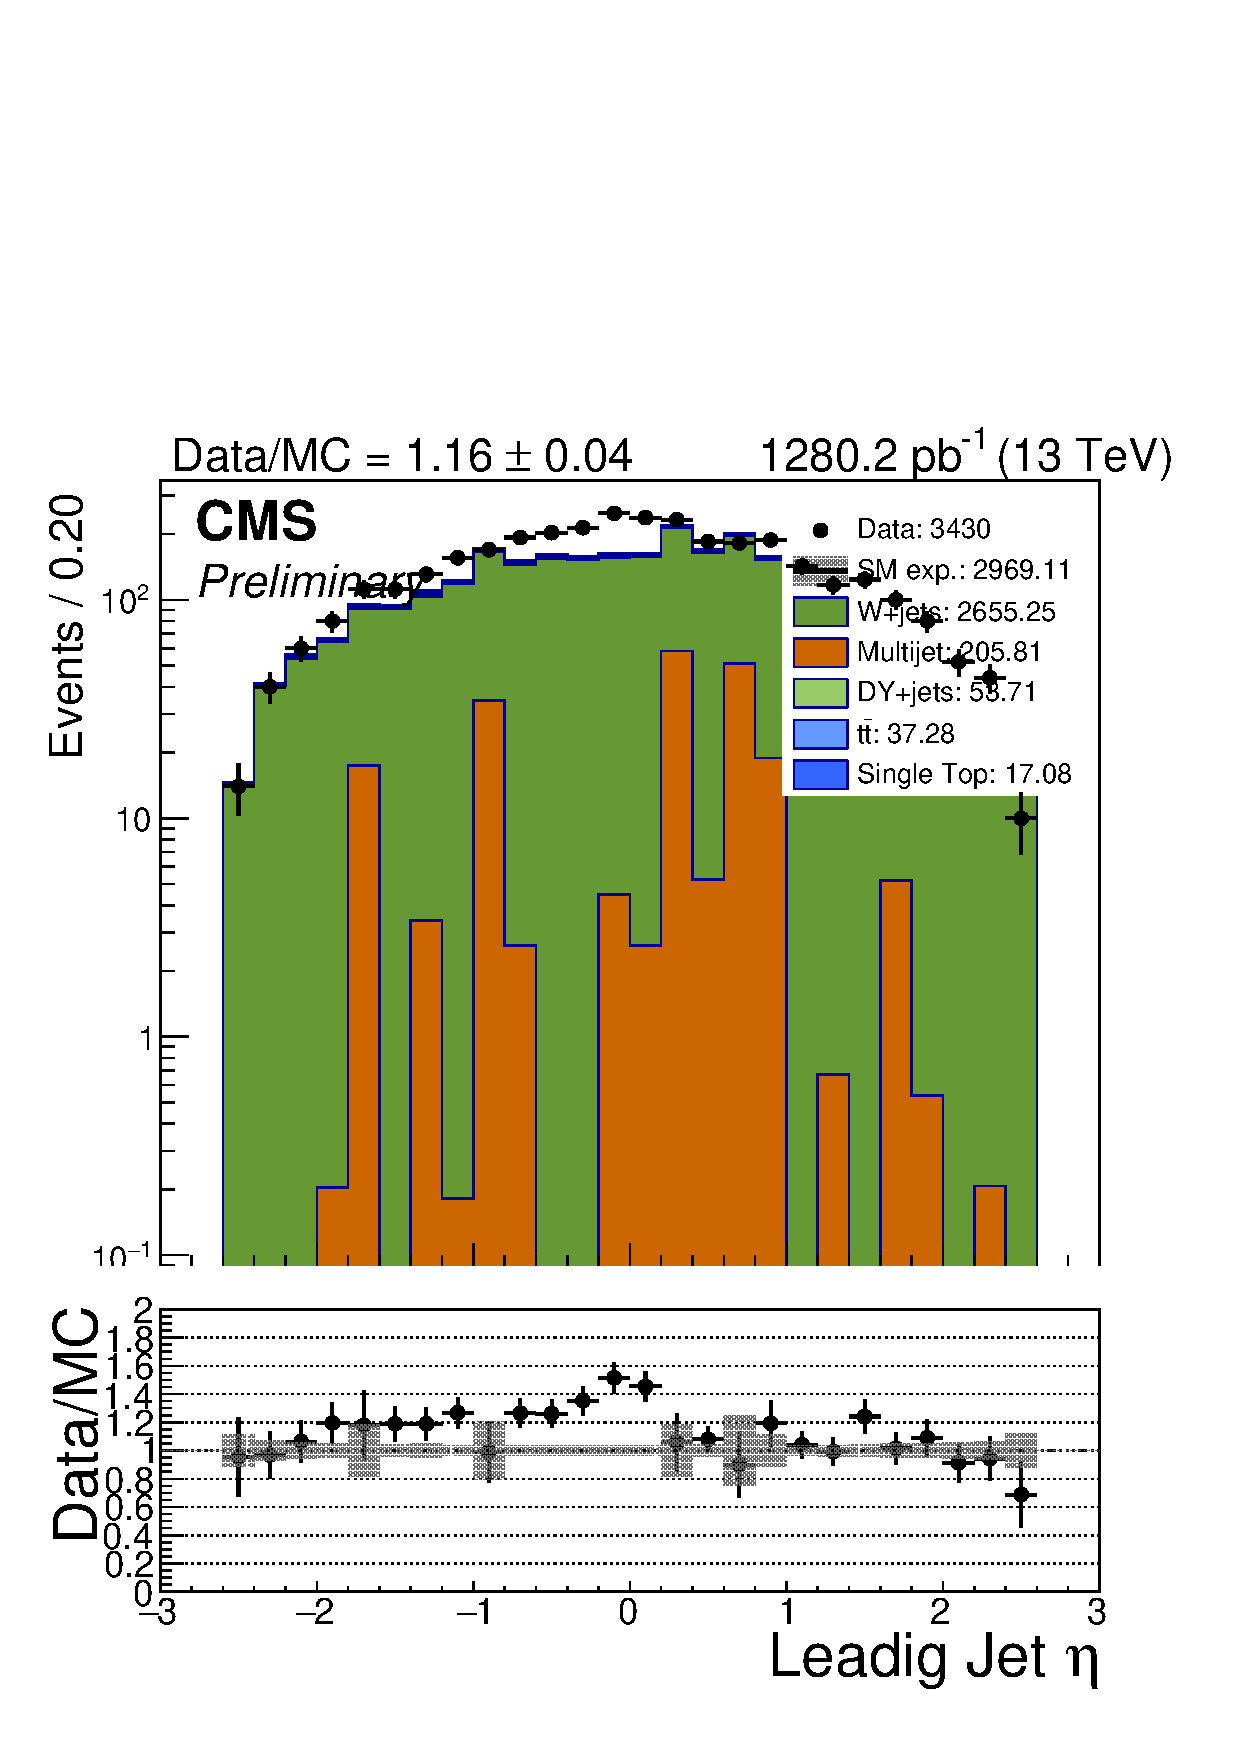
\includegraphics[width=0.5\textwidth]{figures/distributions/SingleEle/jet_eta[0]_eq1j.pdf}} \\
%        \subfigure {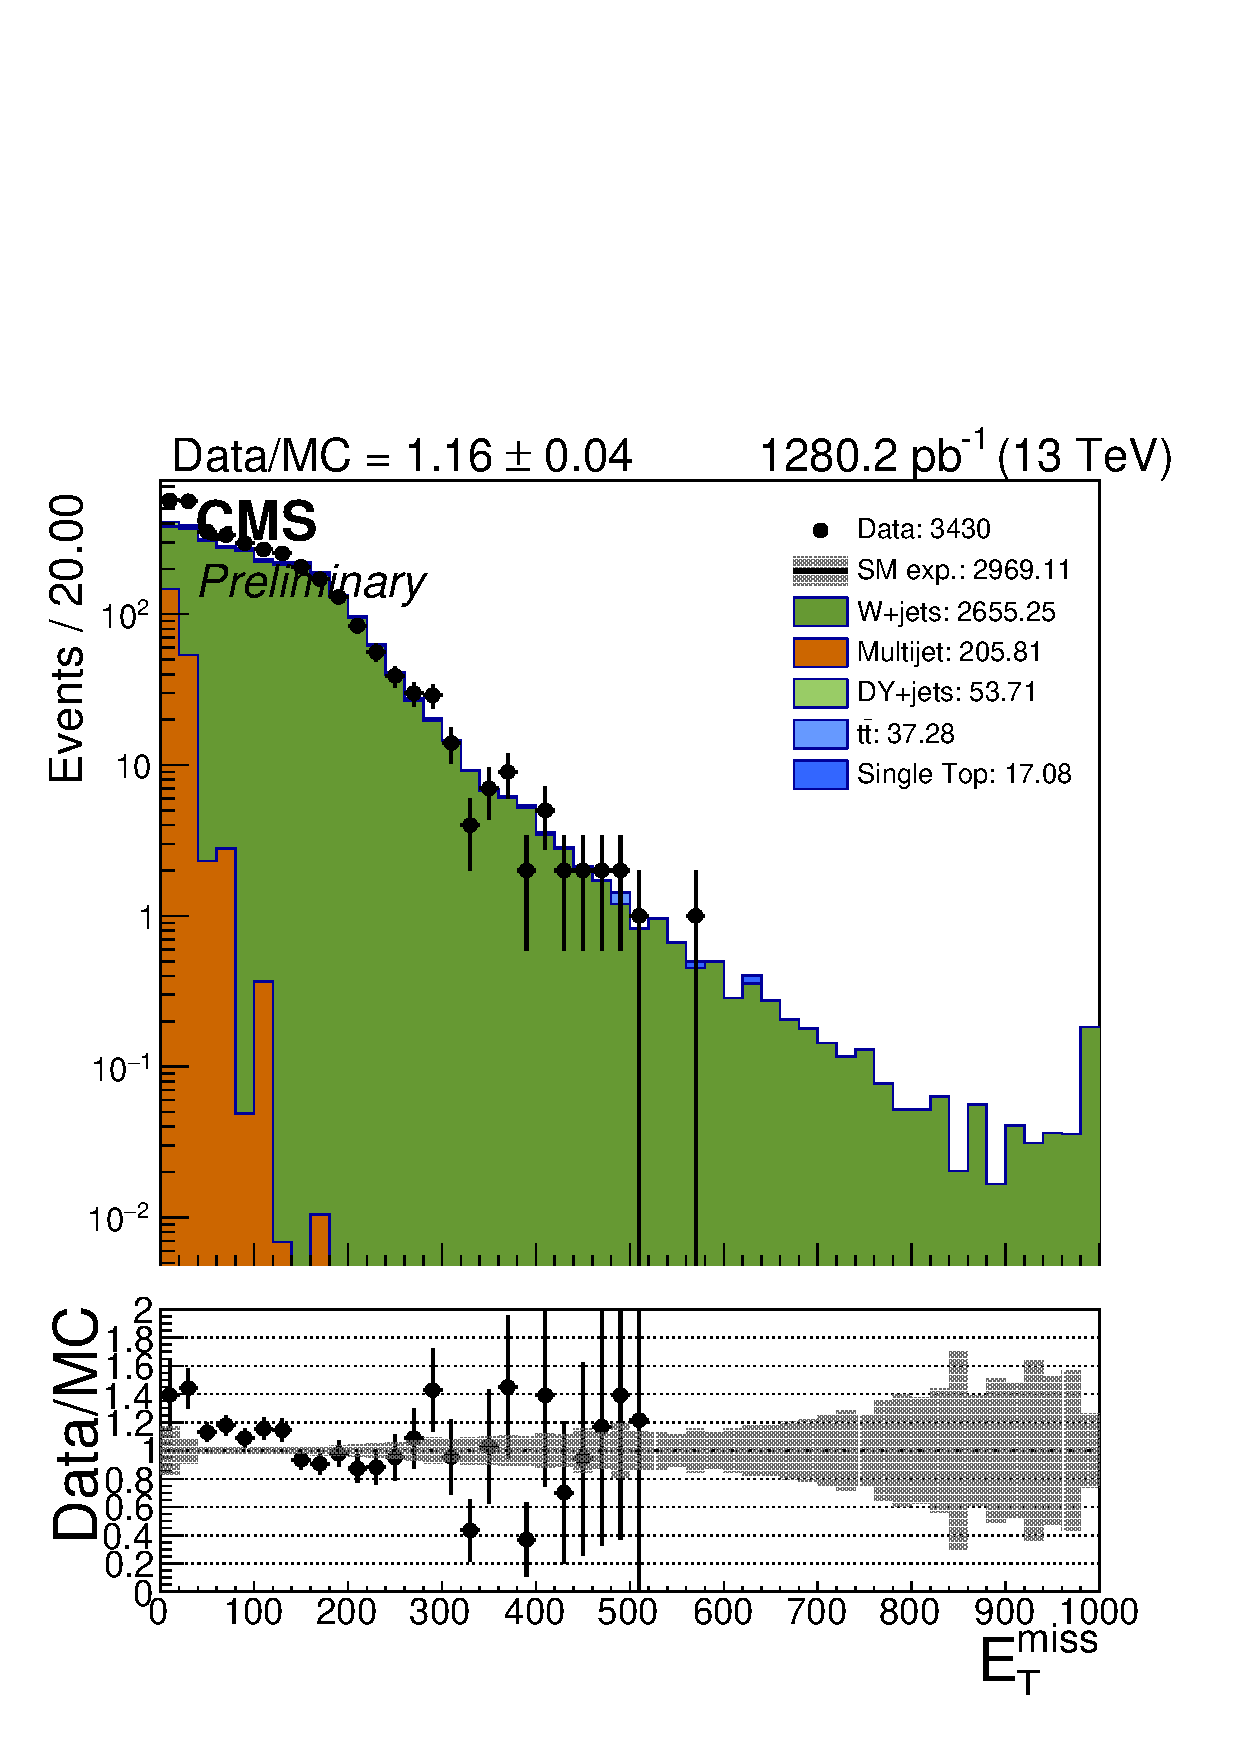
\includegraphics[width=0.5\textwidth]{figures/distributions/SingleEle/met_pt_eq1j.pdf}} ~~
%        \subfigure {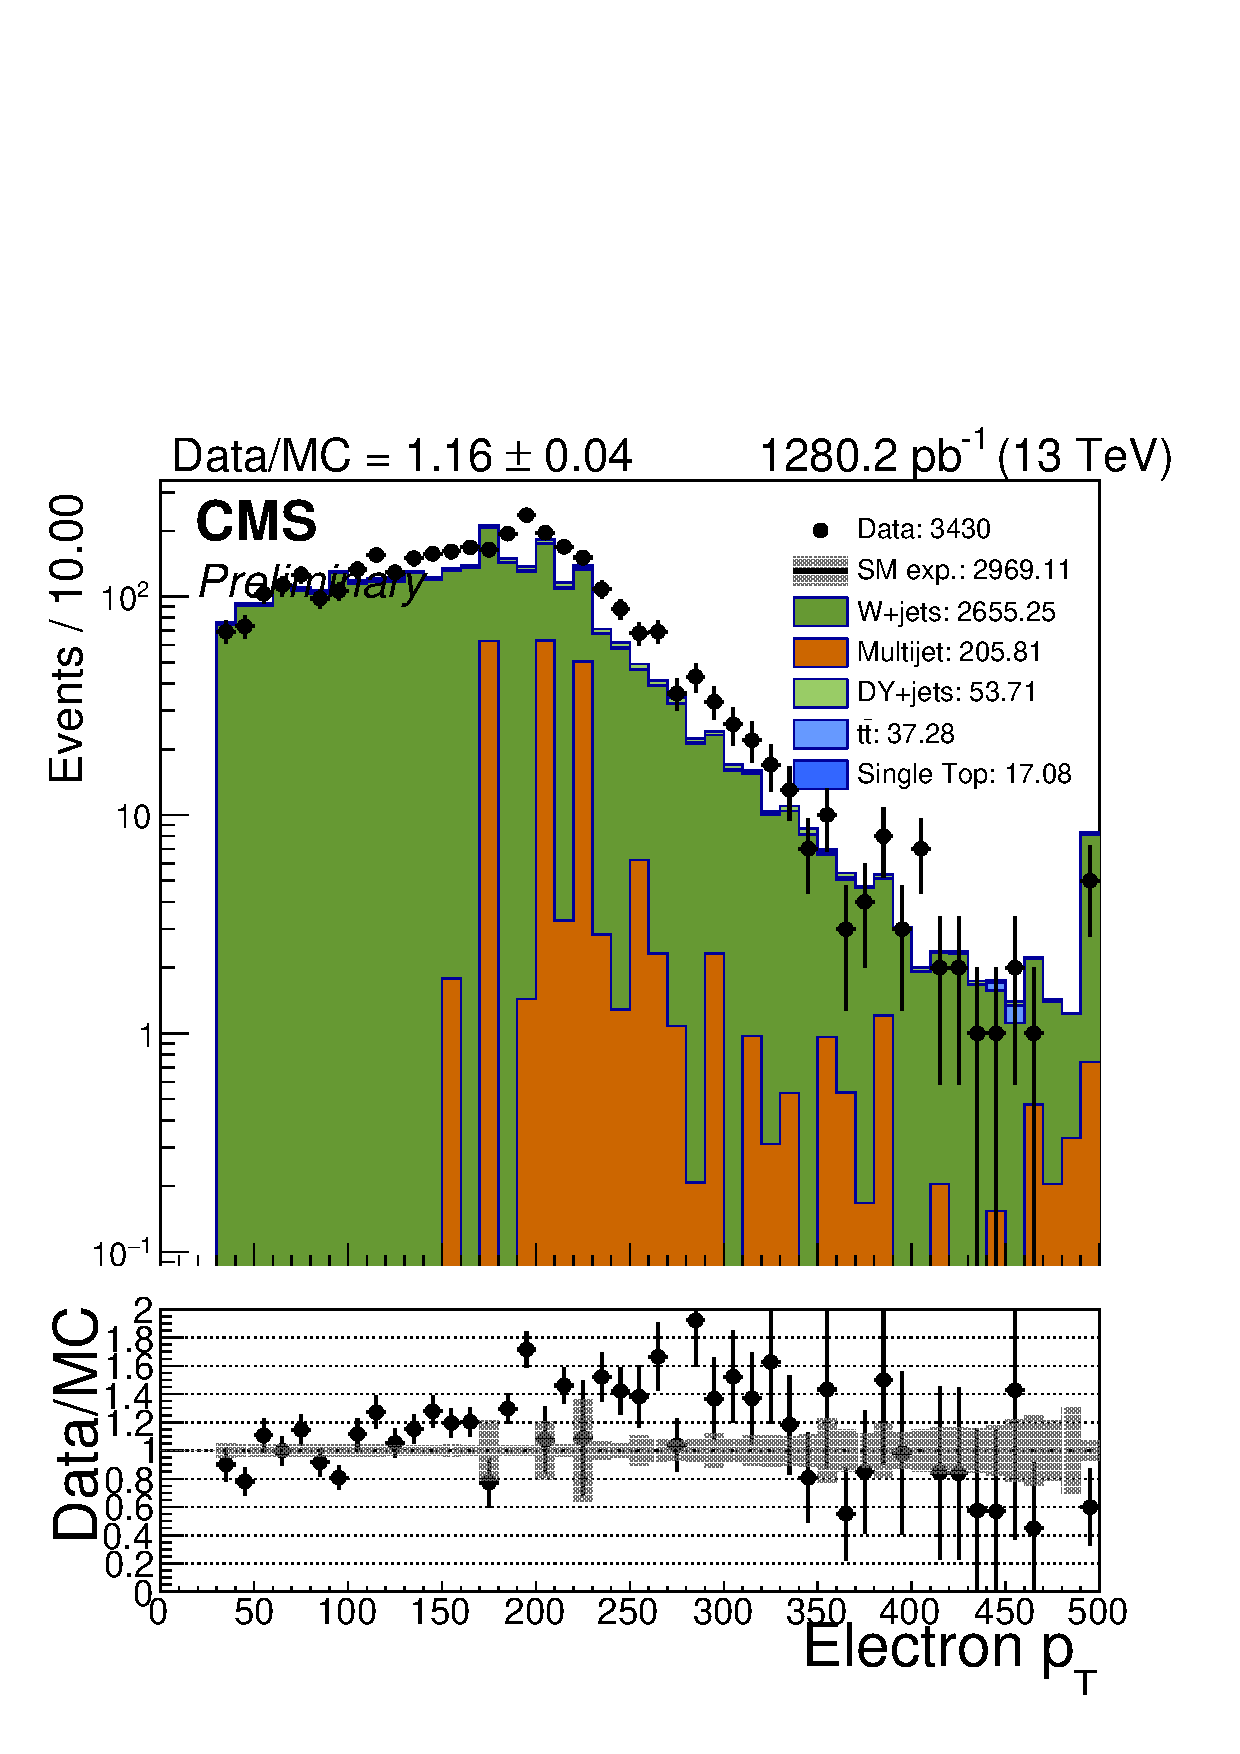
\includegraphics[width=0.5\textwidth]{figures/distributions/SingleEle/ele_pt[0]_eq1j.pdf}} \\
%        \caption{Key analysis variables for single electron control region (monojet bins)}
%        \label{fig:distribution_singleele_mono}
%    \end{center}
%\end{figure}
%
%\newpage
%\subsection{Yields and distributions for the $\mu\mu$ + jets control sample}
%
%\begin{figure}
%    \begin{center}
%        \subfigure {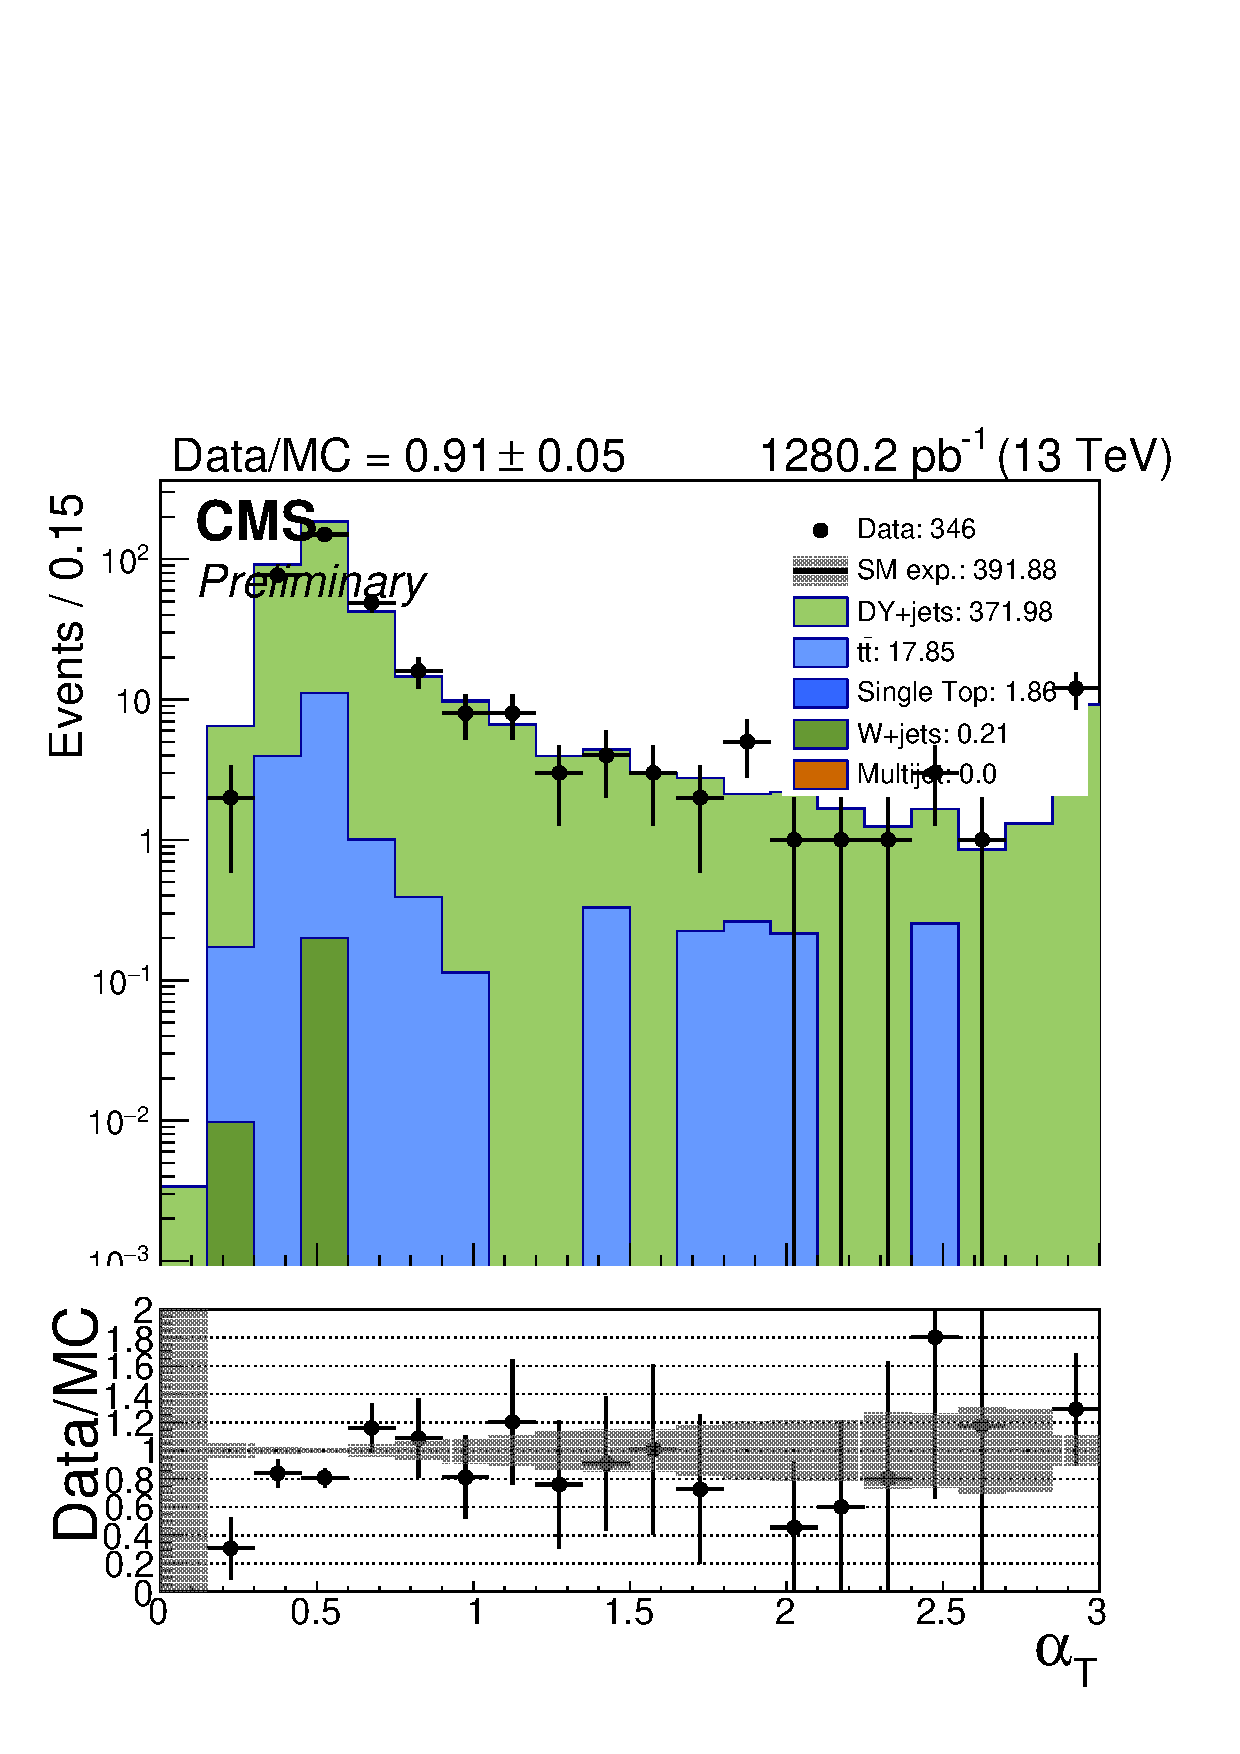
\includegraphics[width=0.5\textwidth]{figures/distributions/DoubleEle/alphaT_sym.pdf}} ~~
%        \subfigure {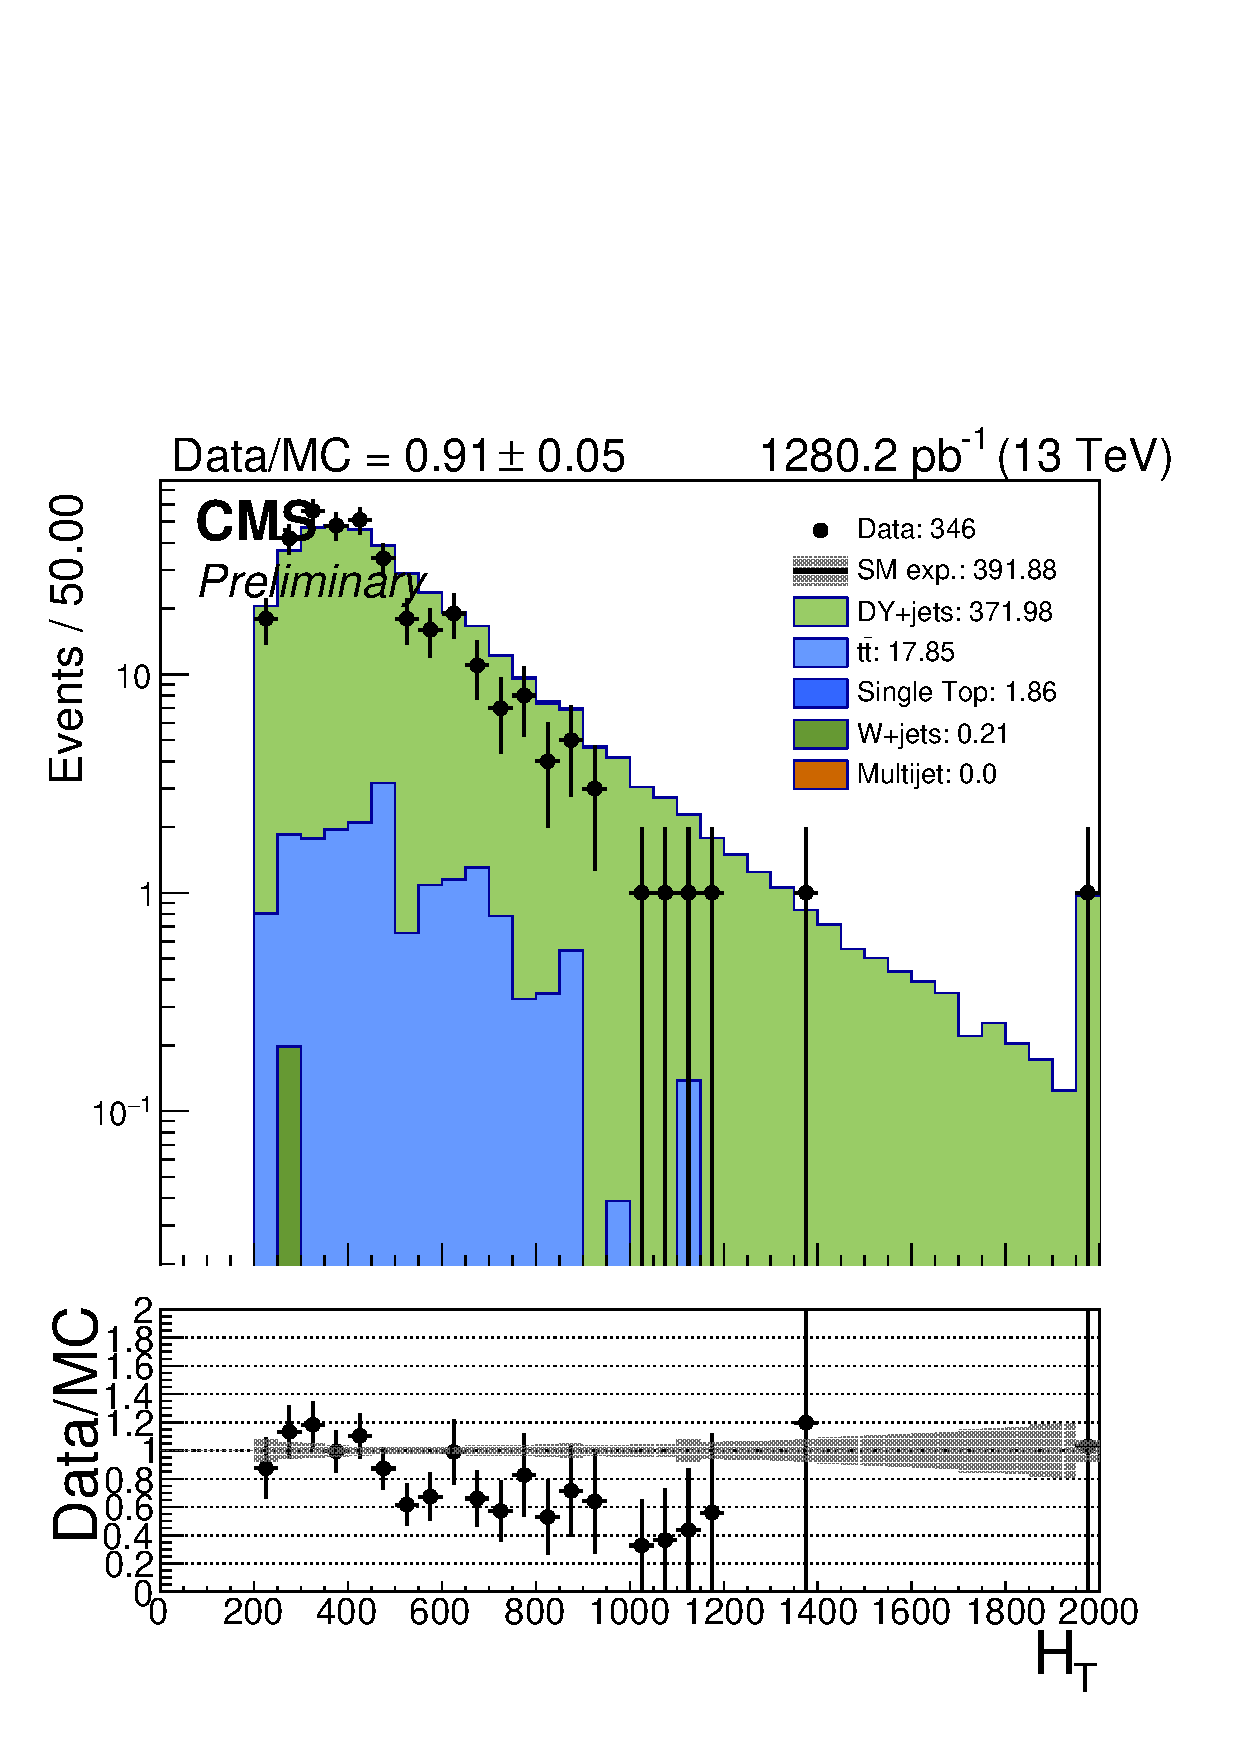
\includegraphics[width=0.5\textwidth]{figures/distributions/DoubleEle/ht40_sym.pdf}} \\
%        \subfigure {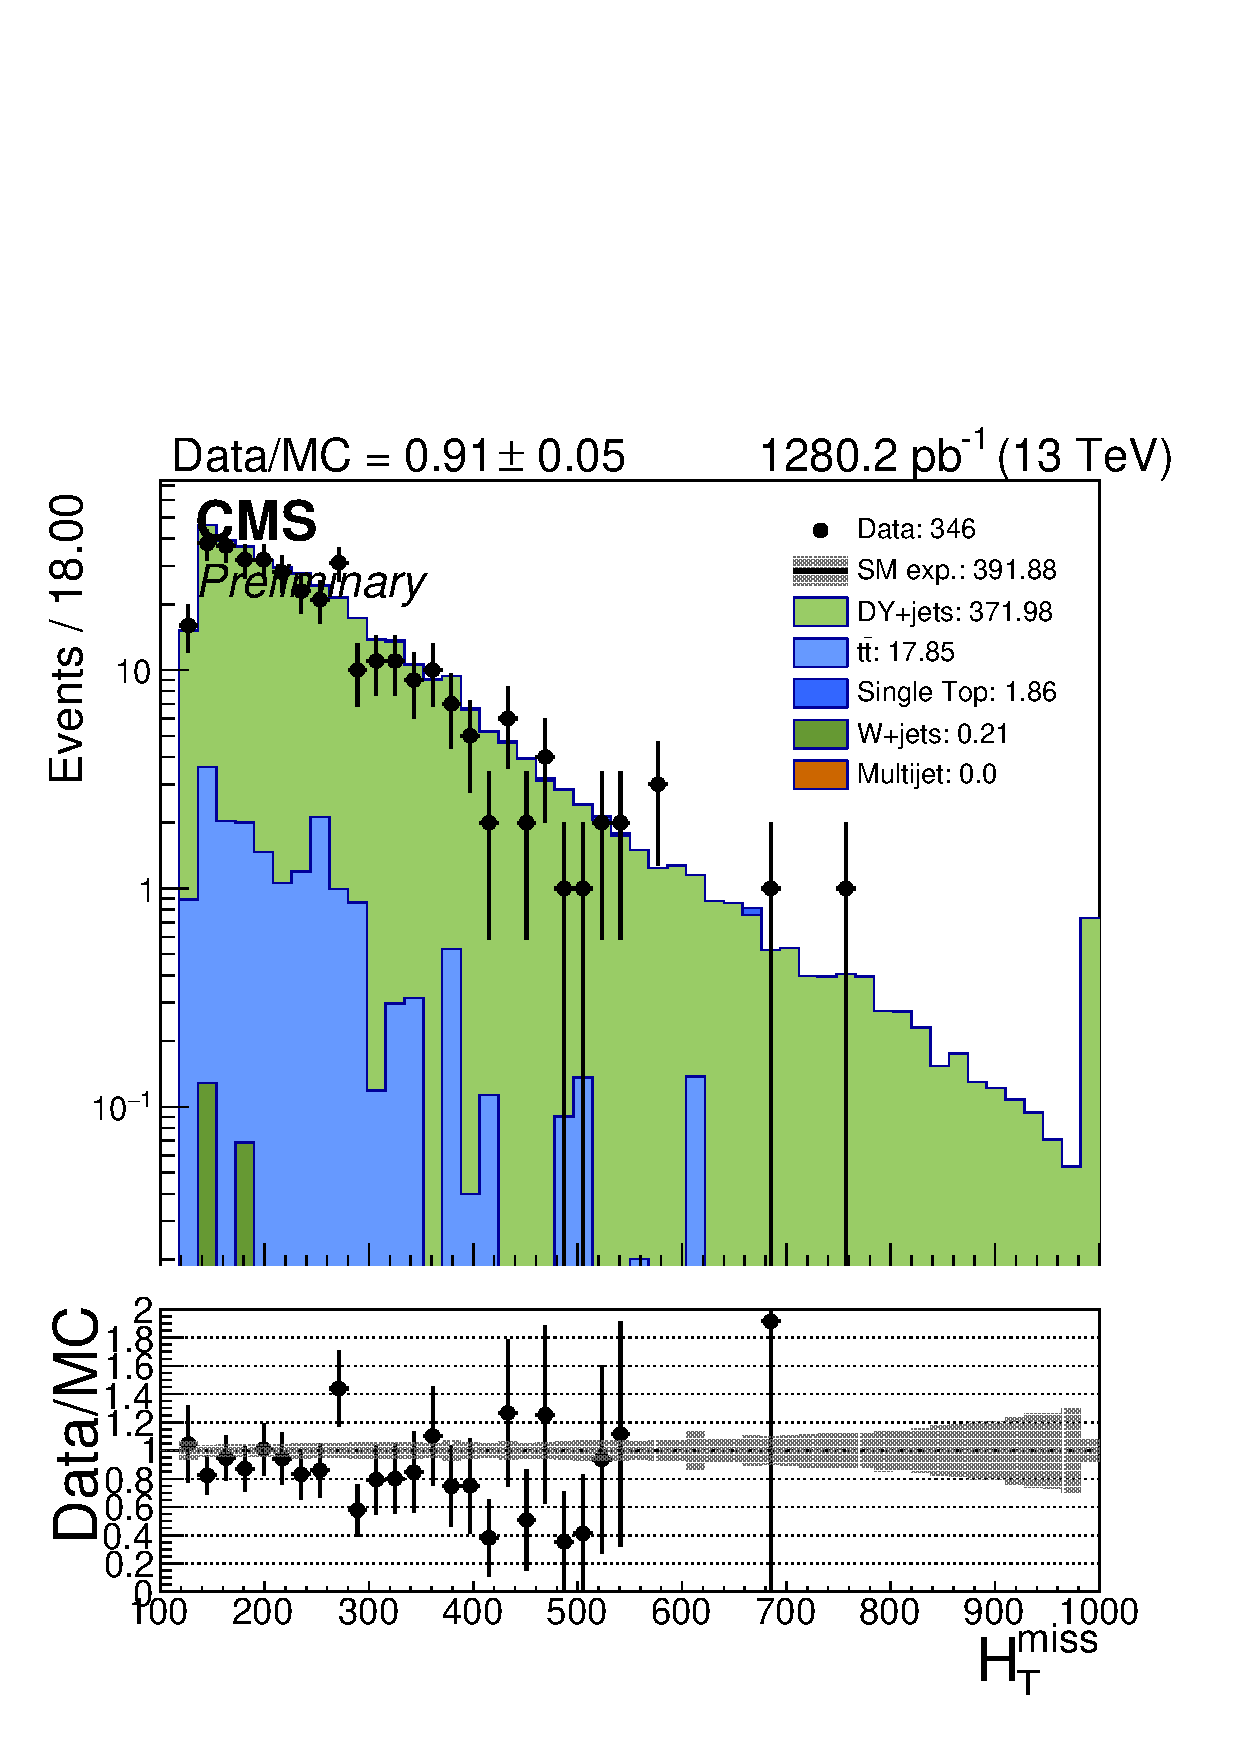
\includegraphics[width=0.5\textwidth]{figures/distributions/DoubleEle/mht40_pt_sym.pdf}} ~~
%        \subfigure {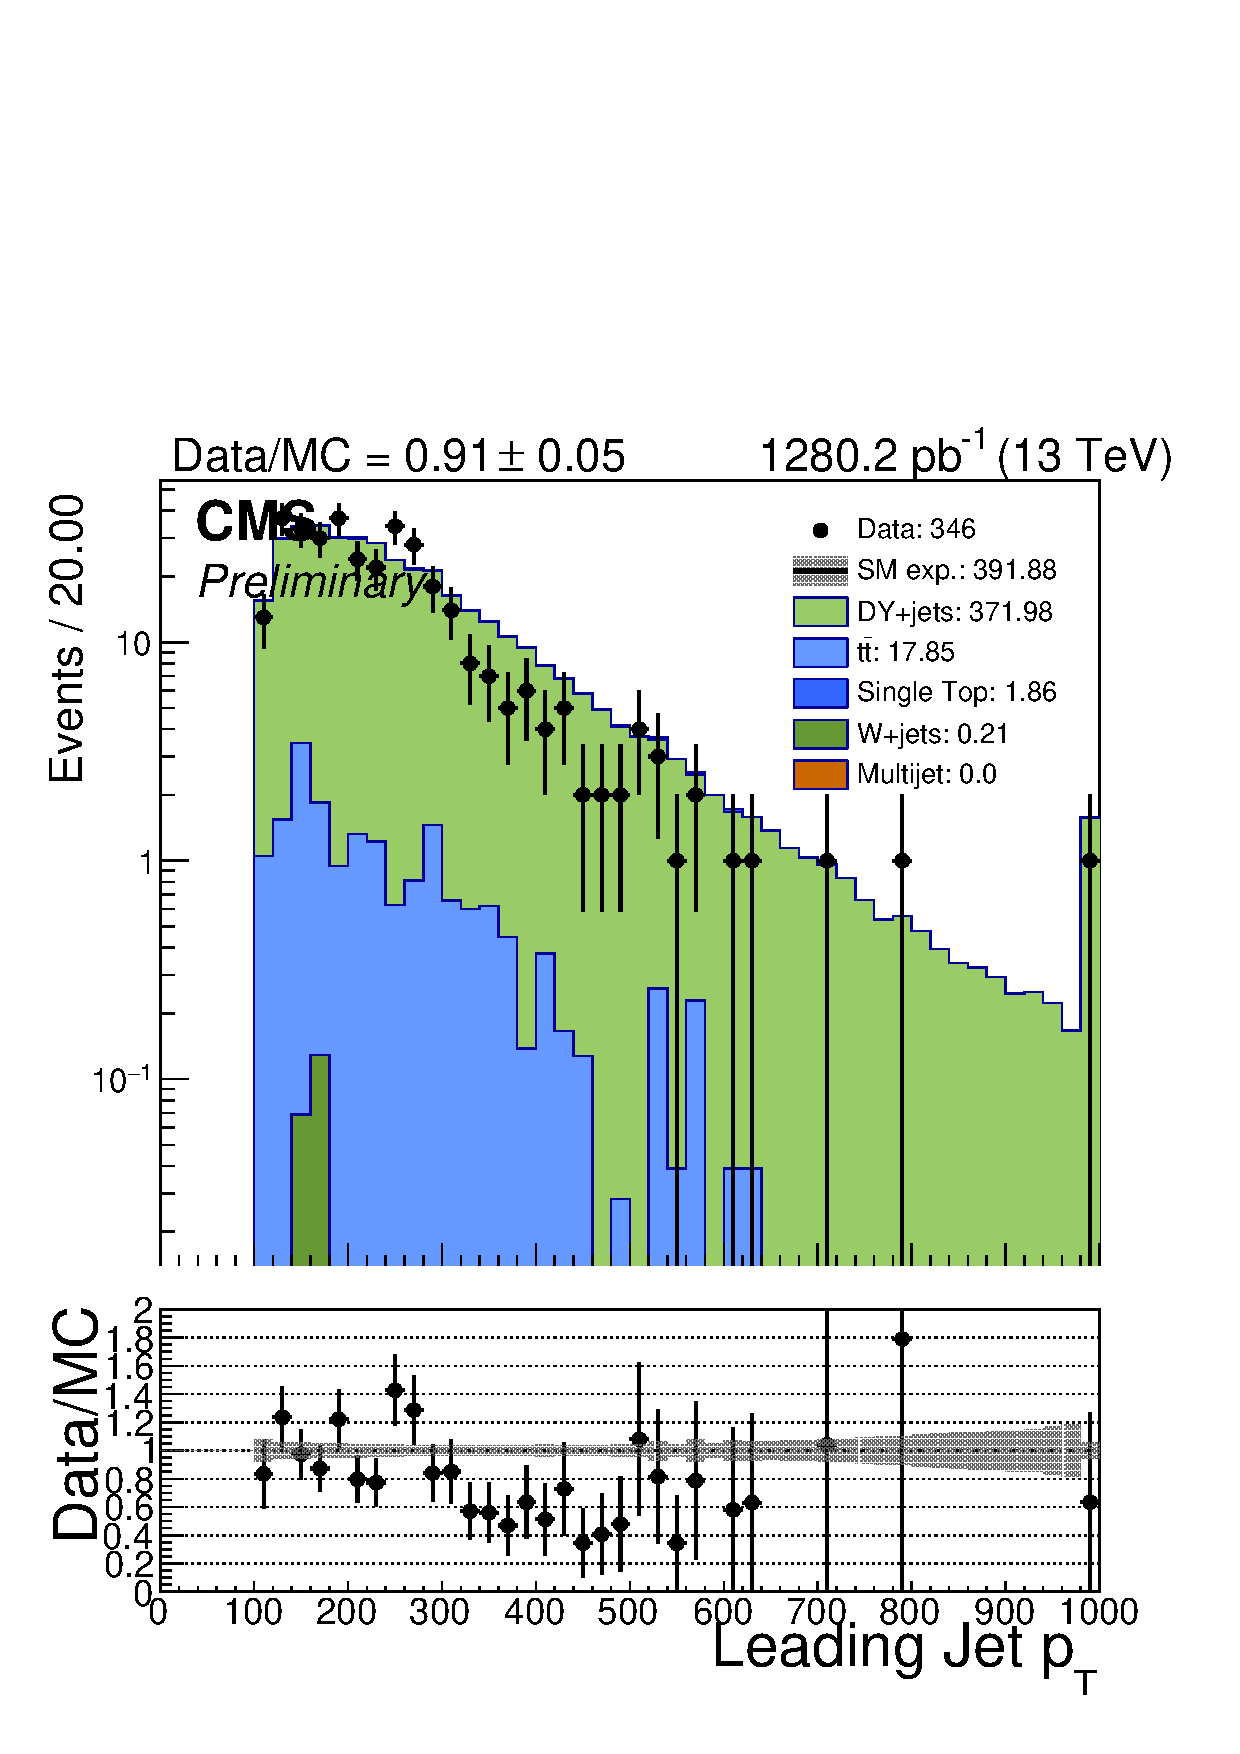
\includegraphics[width=0.5\textwidth]{figures/distributions/DoubleEle/jet_pt[0]_sym.pdf}} \\
%        \caption{Key analysis variables for double electron control region (symmetric \njet bins)}
%        \label{fig:distribution_doubleele_sym}
%    \end{center}
%\end{figure}
%
%\begin{figure}
%    \begin{center}
%        \subfigure {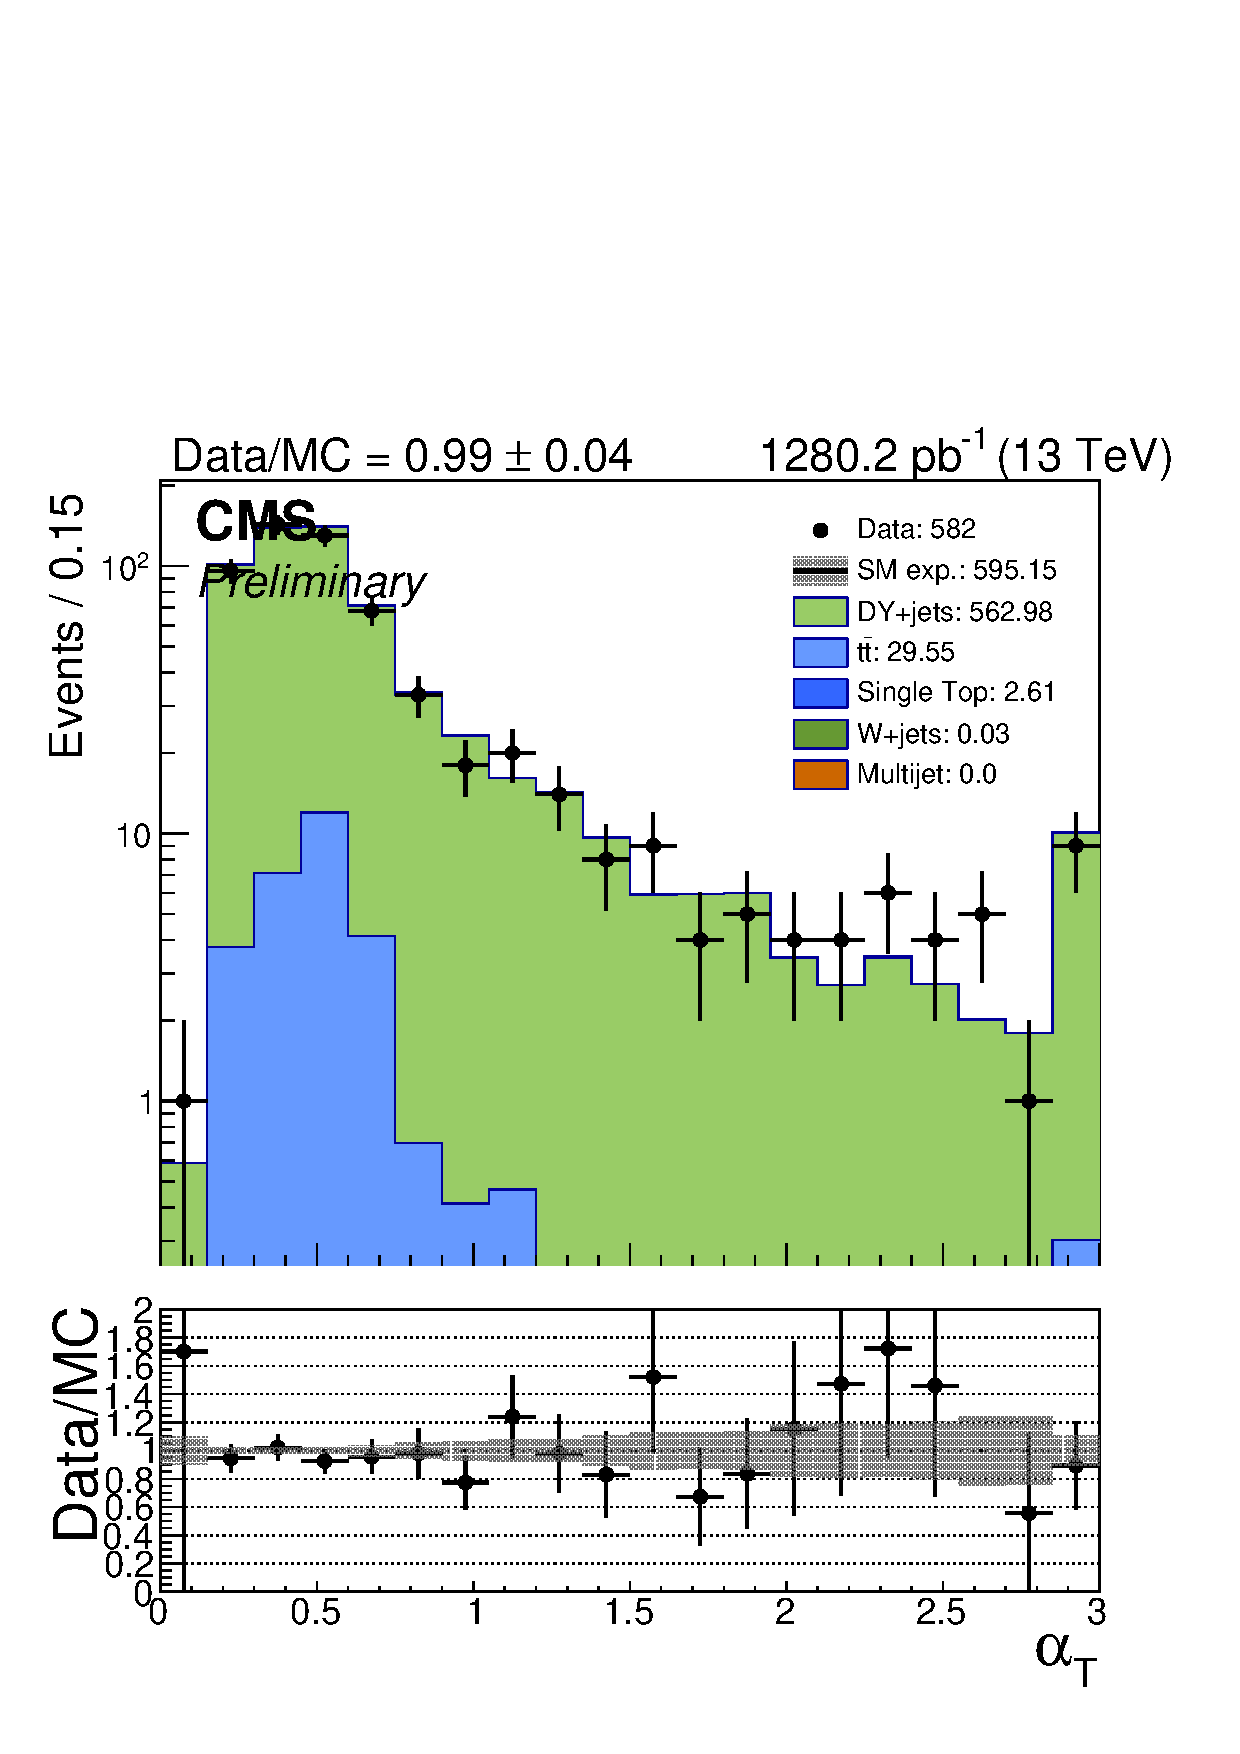
\includegraphics[width=0.5\textwidth]{figures/distributions/DoubleEle/alphaT_asym.pdf}} ~~
%        \subfigure {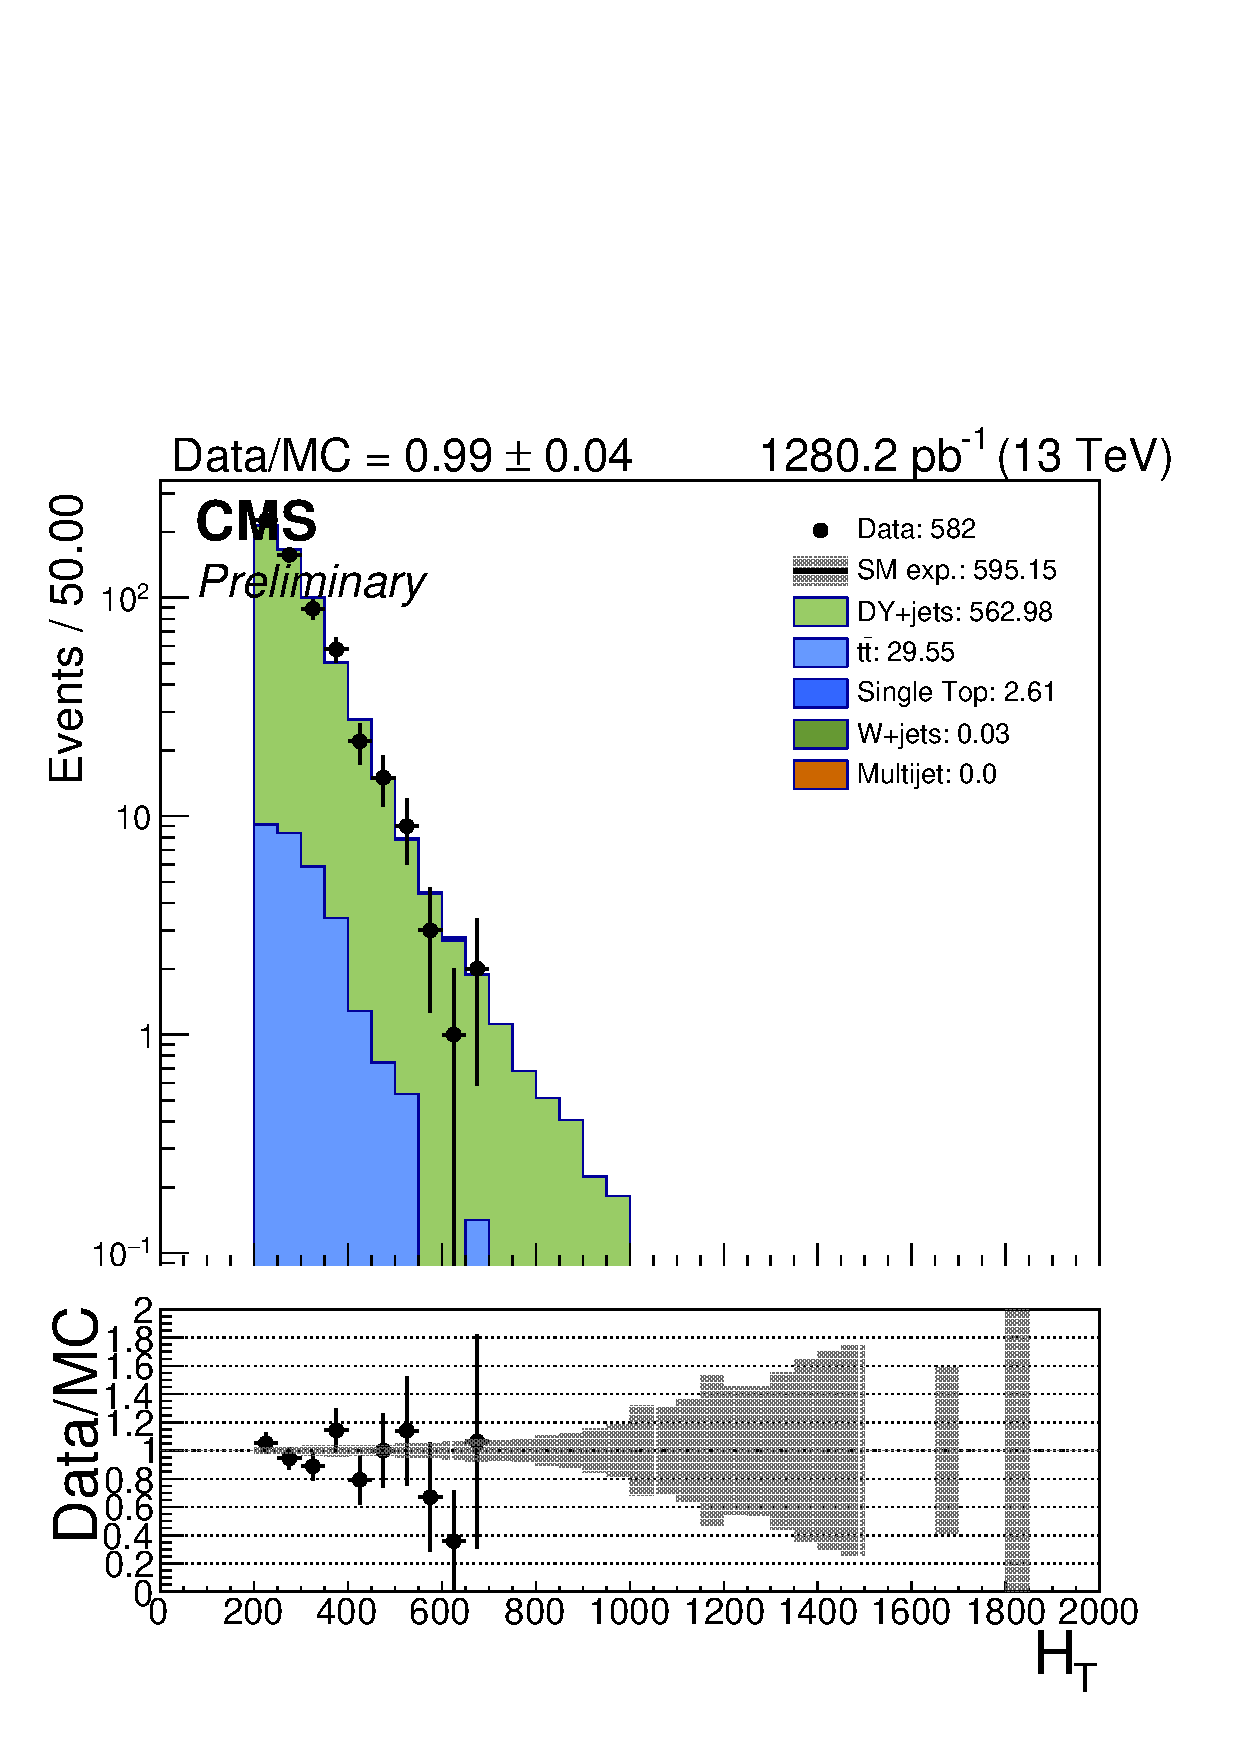
\includegraphics[width=0.5\textwidth]{figures/distributions/DoubleEle/ht40_asym.pdf}} \\
%        \subfigure {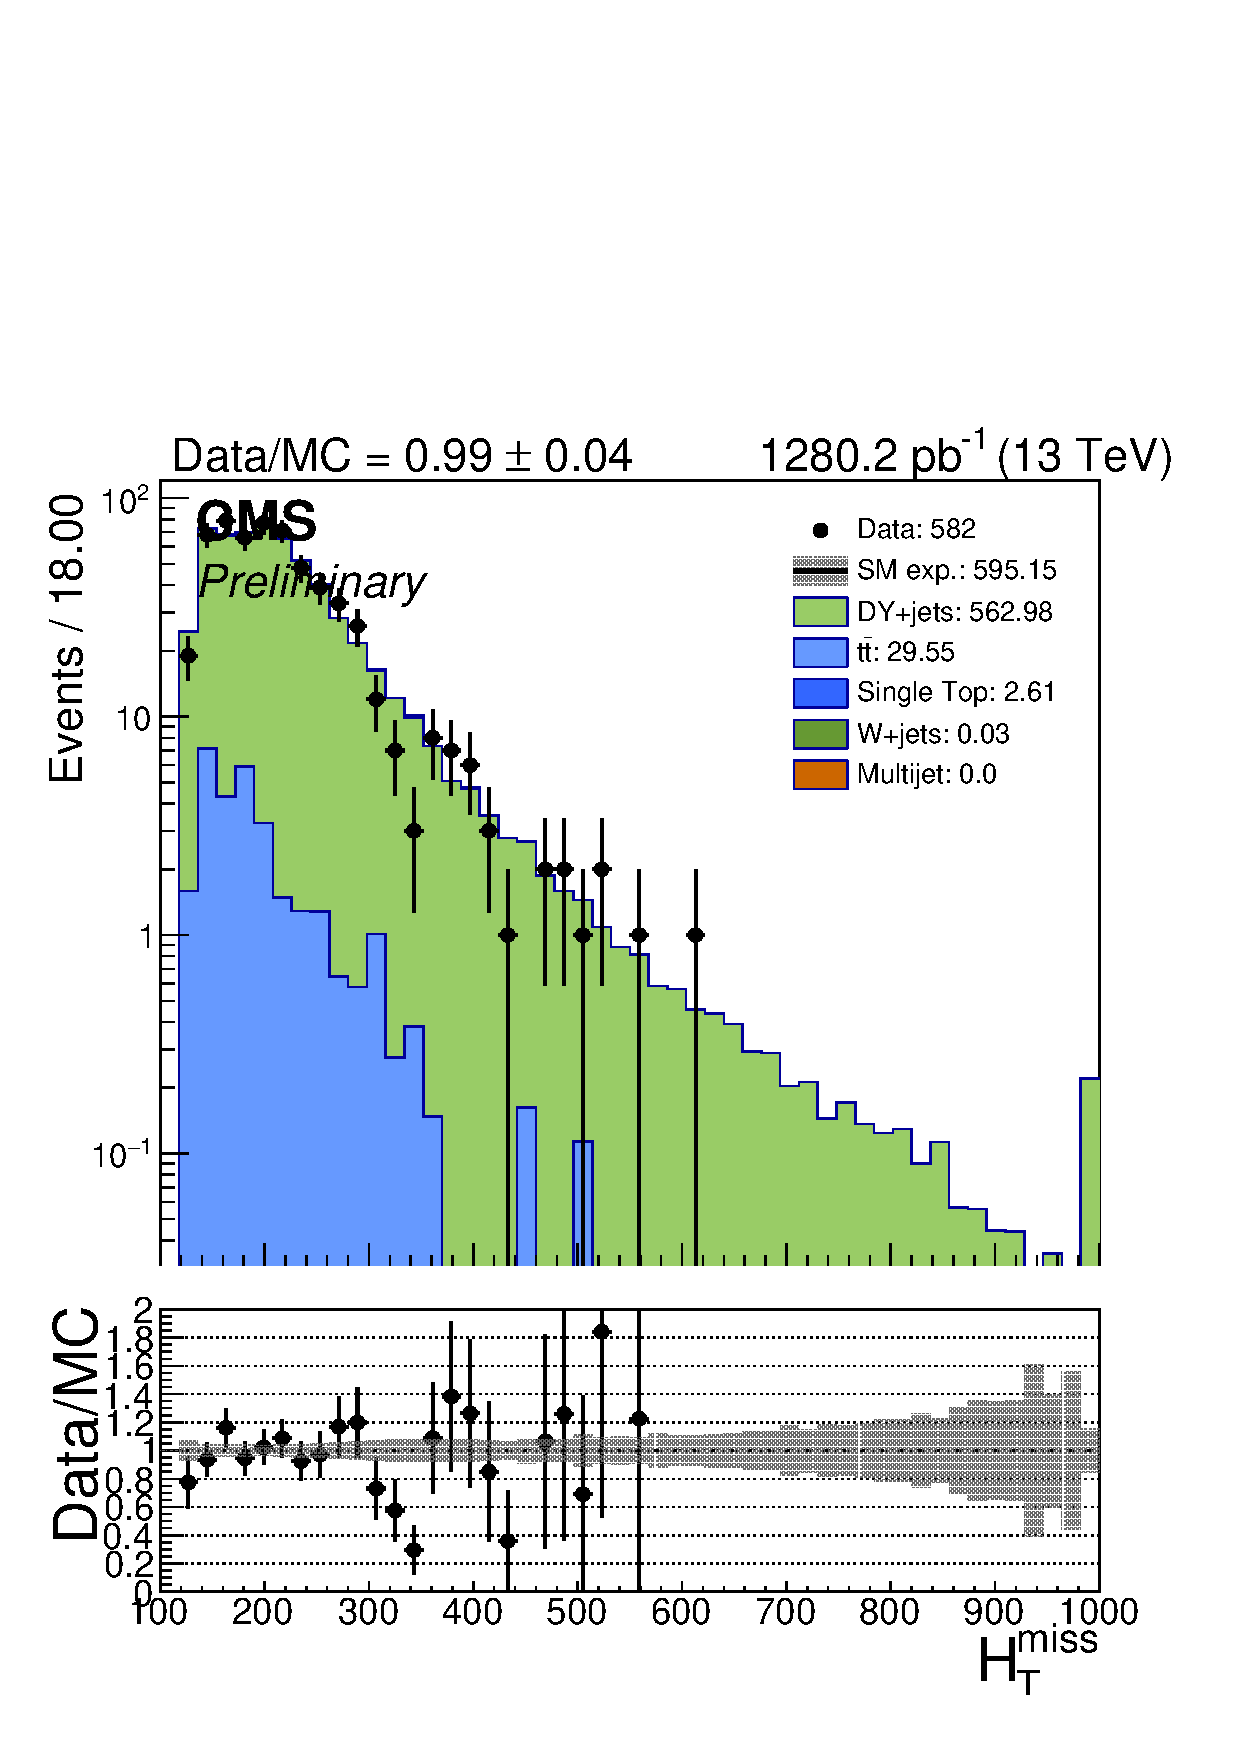
\includegraphics[width=0.5\textwidth]{figures/distributions/DoubleEle/mht40_pt_asym.pdf}} ~~
%        \subfigure {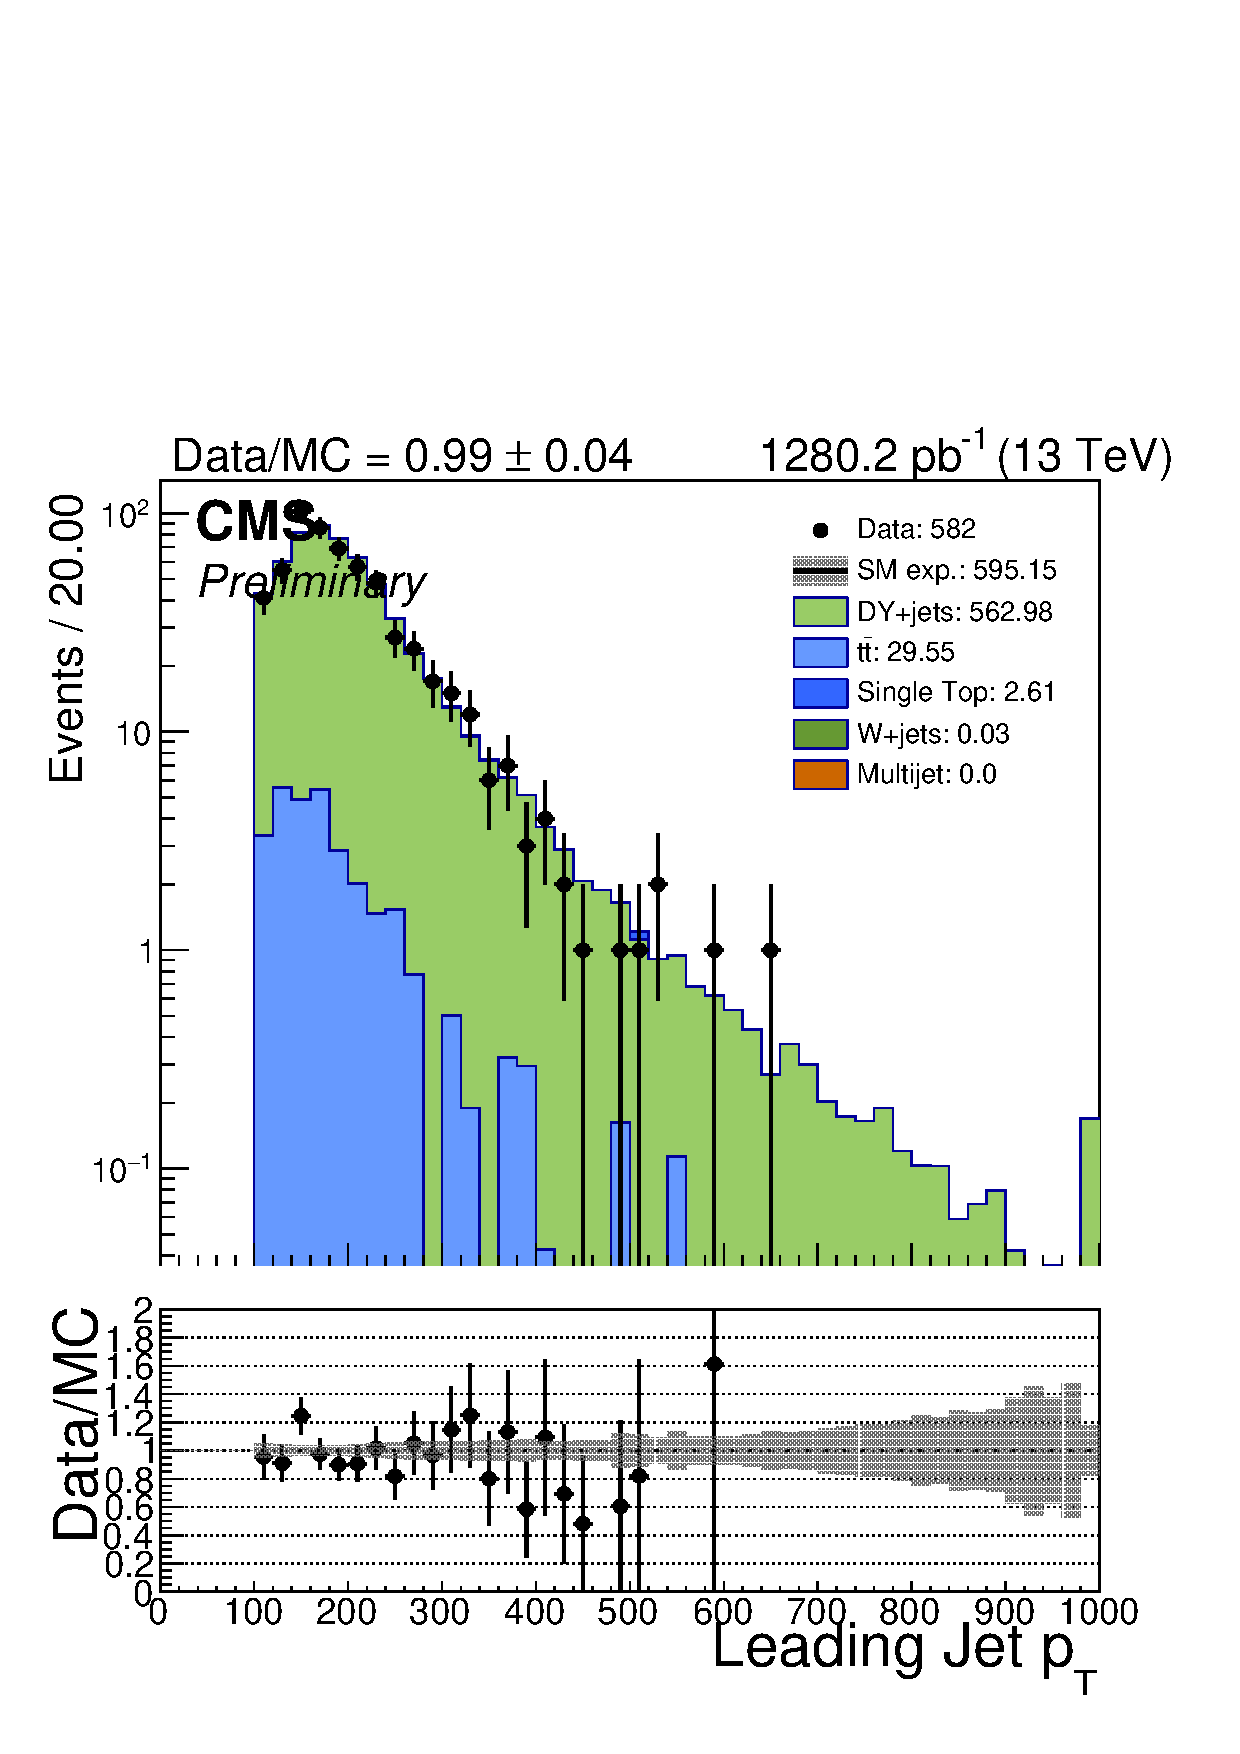
\includegraphics[width=0.5\textwidth]{figures/distributions/DoubleEle/jet_pt[0]_asym.pdf}} \\
%        \caption{Key analysis variables for double electron control region (asymmetric \njet bins)}
%        \label{fig:distribution_doubleele_asym}
%    \end{center}
%\end{figure}
%
%\begin{figure}
%    \begin{center} 
%        \subfigure {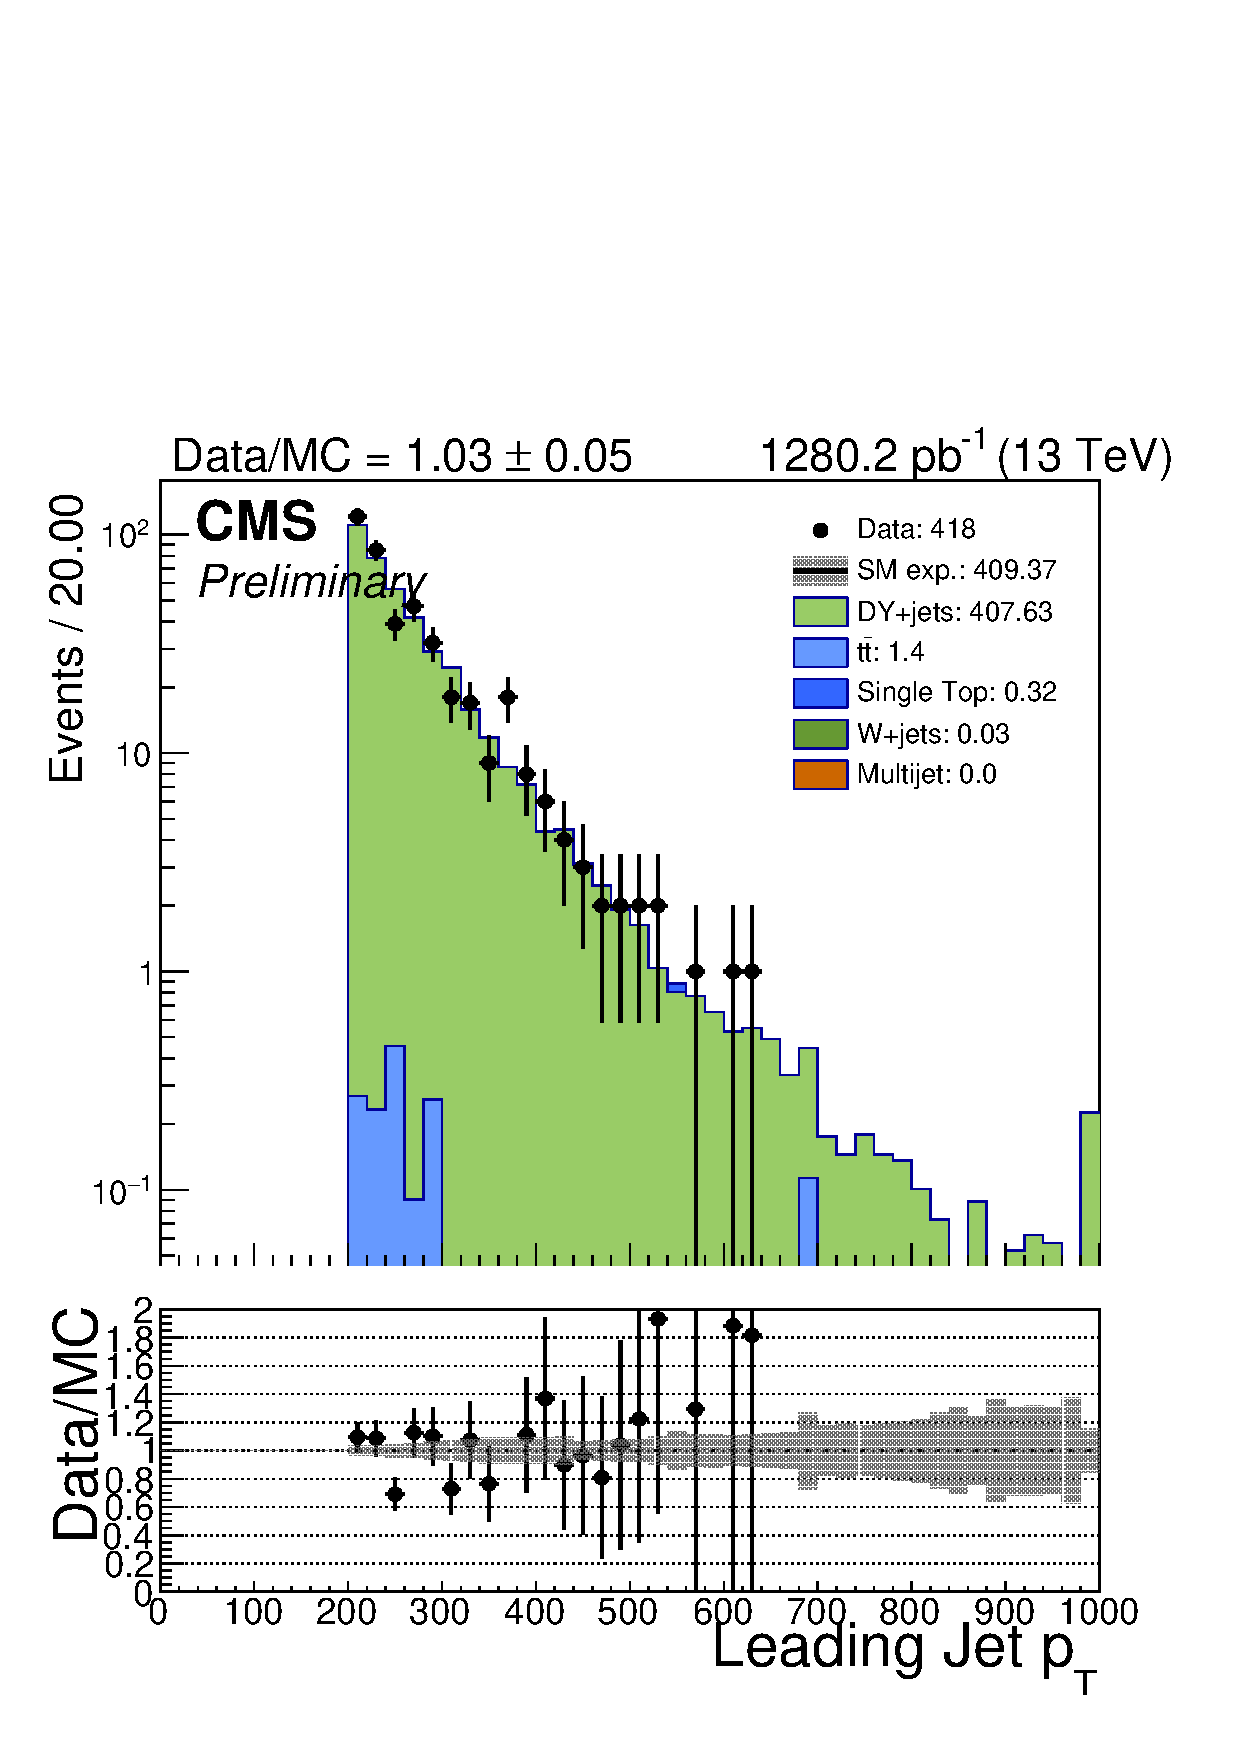
\includegraphics[width=0.5\textwidth]{figures/distributions/DoubleEle/jet_pt[0]_eq1j.pdf}} ~~
%        \subfigure {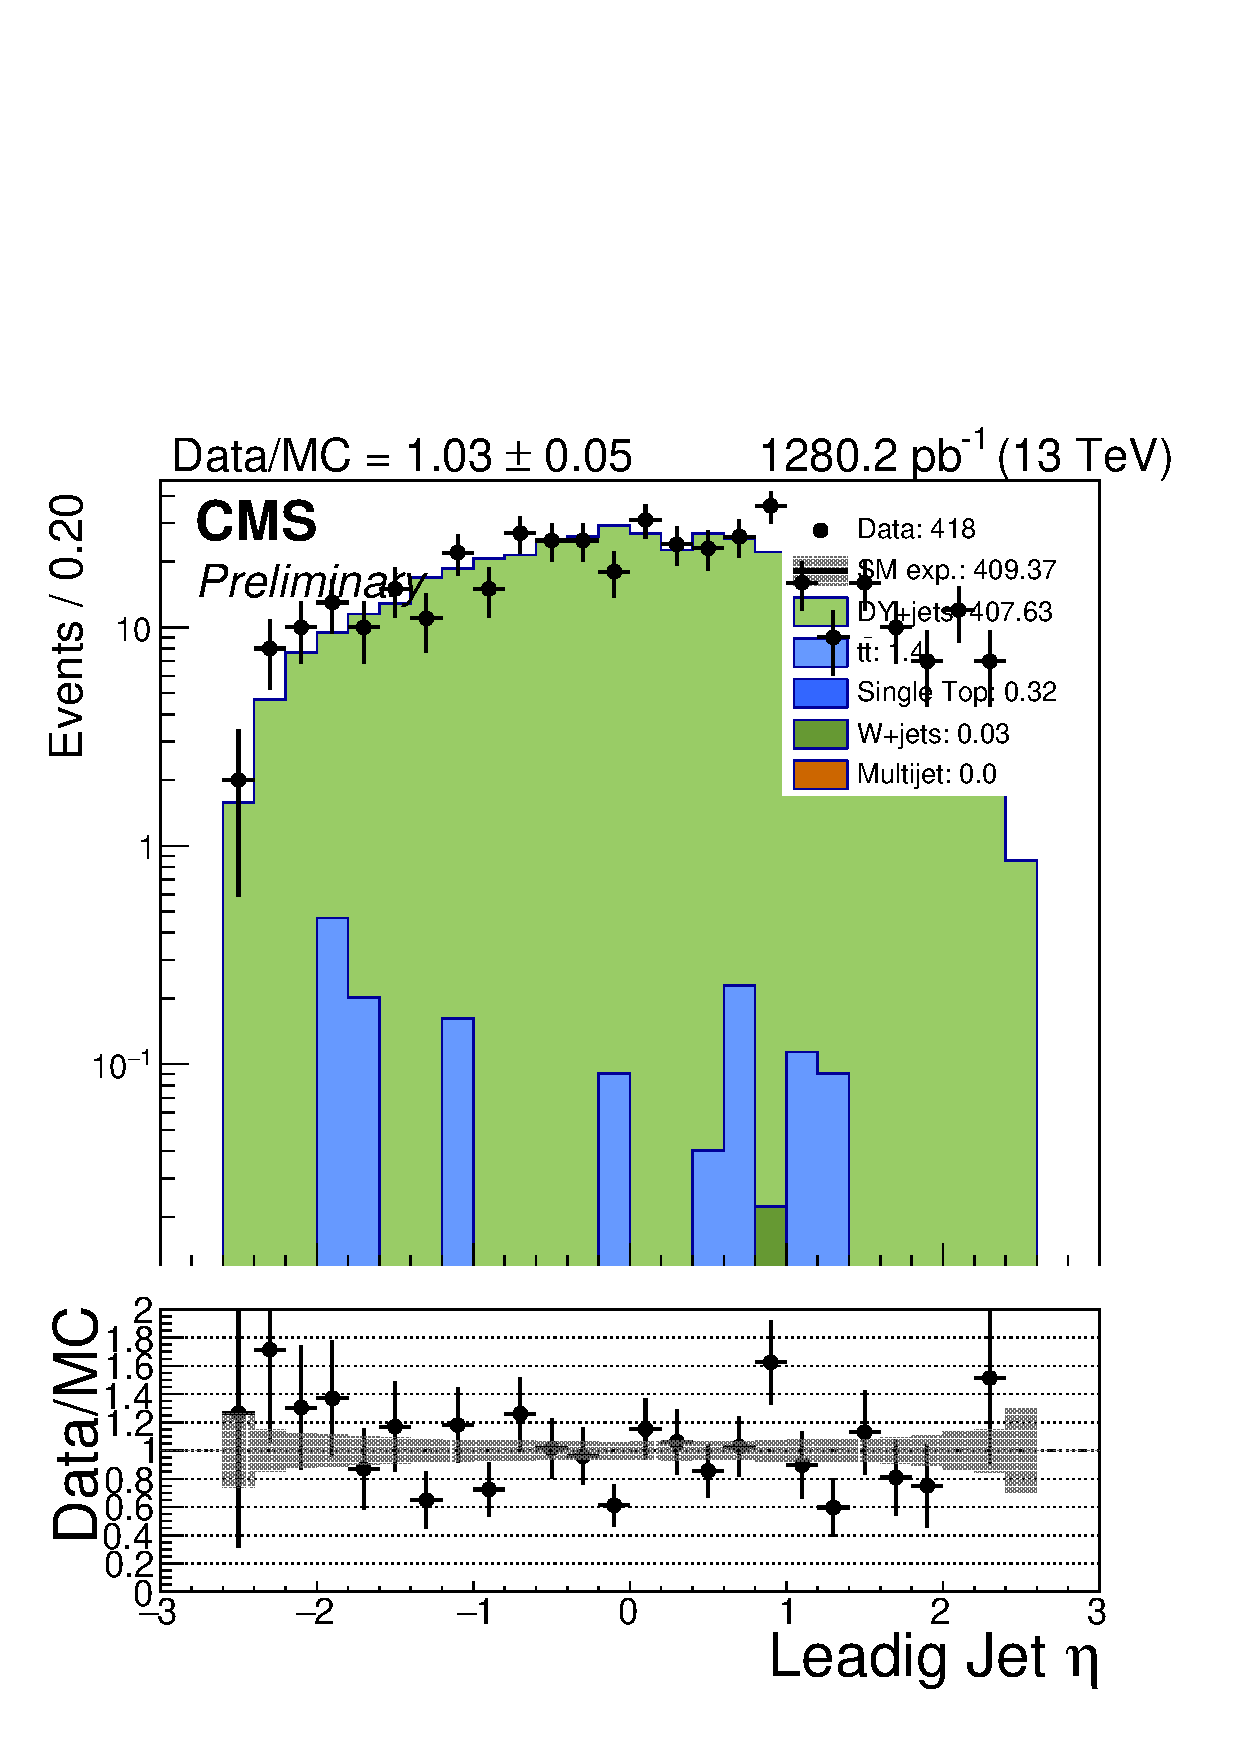
\includegraphics[width=0.5\textwidth]{figures/distributions/DoubleEle/jet_eta[0]_eq1j.pdf}} \\
%        \subfigure {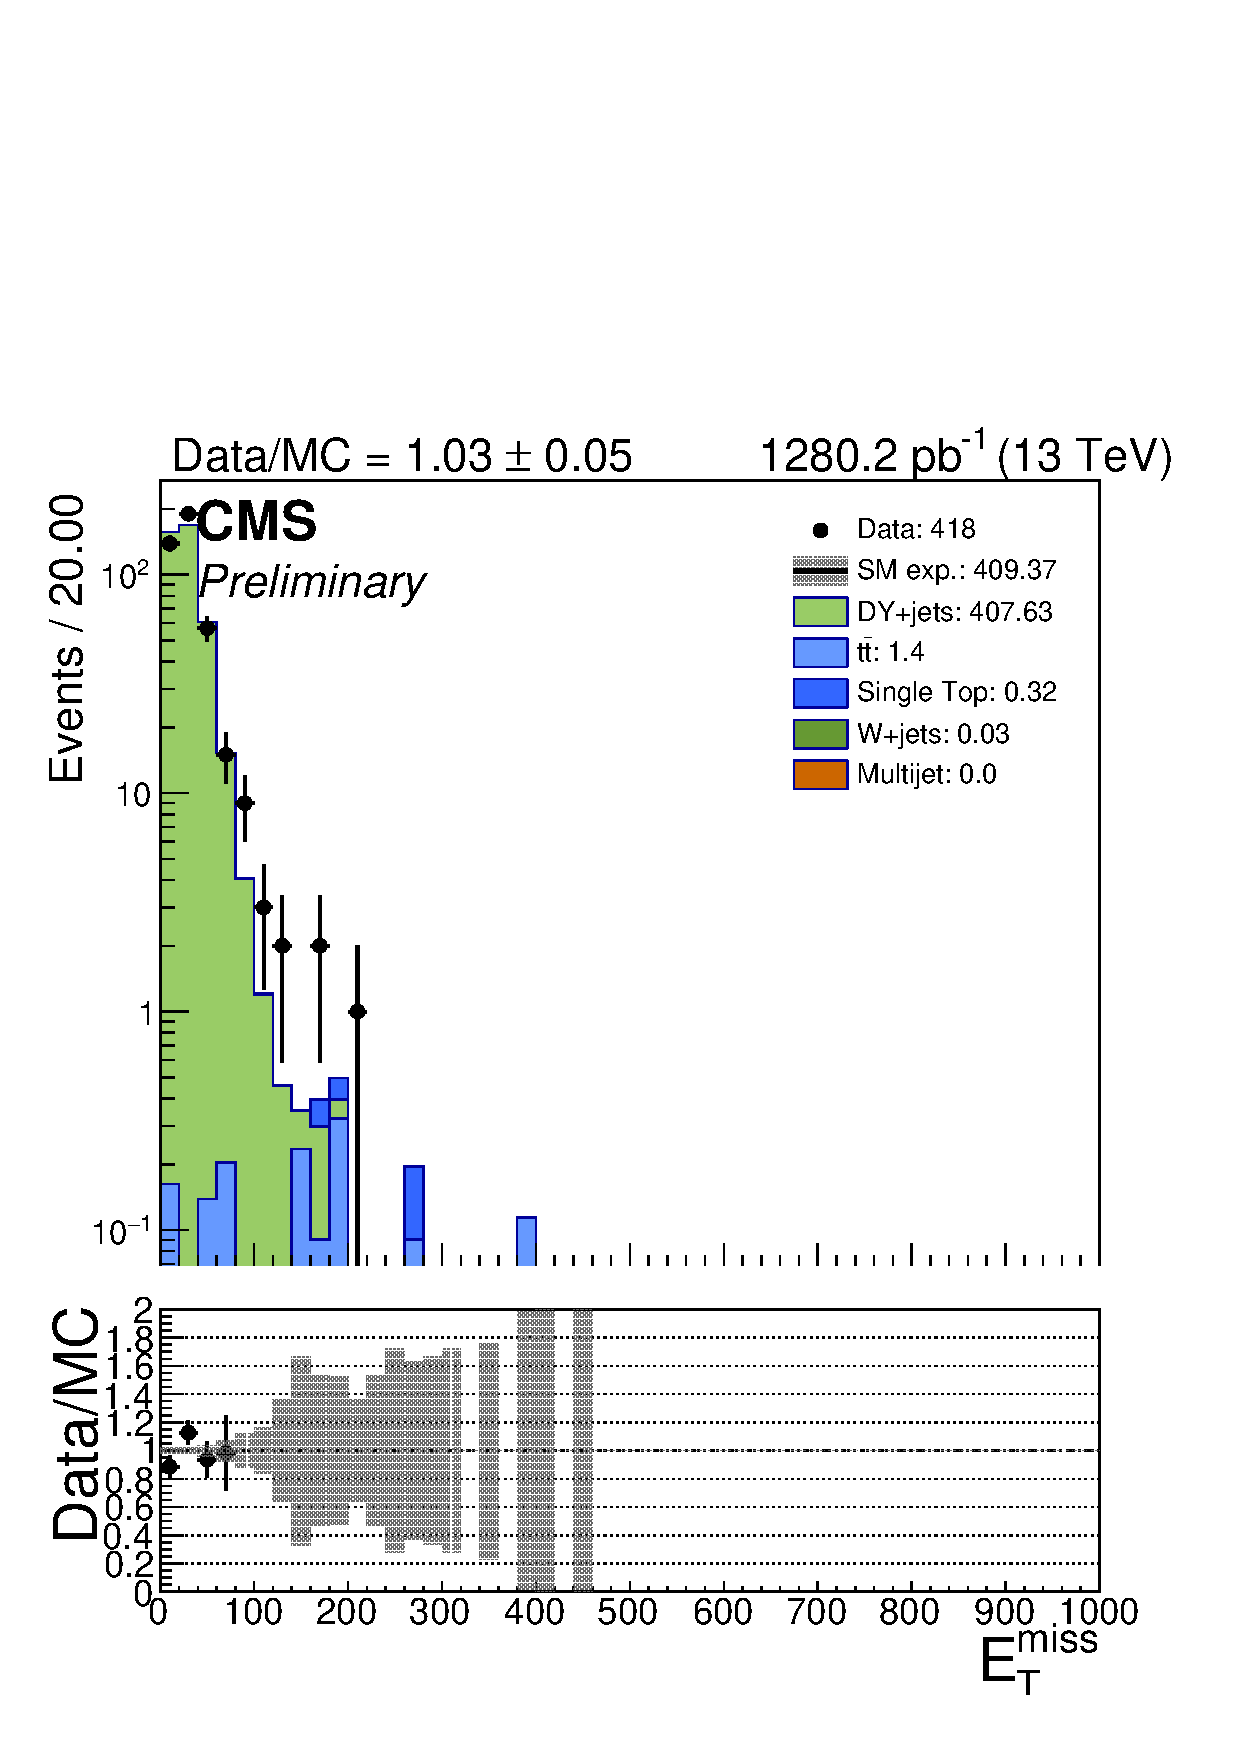
\includegraphics[width=0.5\textwidth]{figures/distributions/DoubleEle/met_pt_eq1j.pdf}} ~~
%        \subfigure {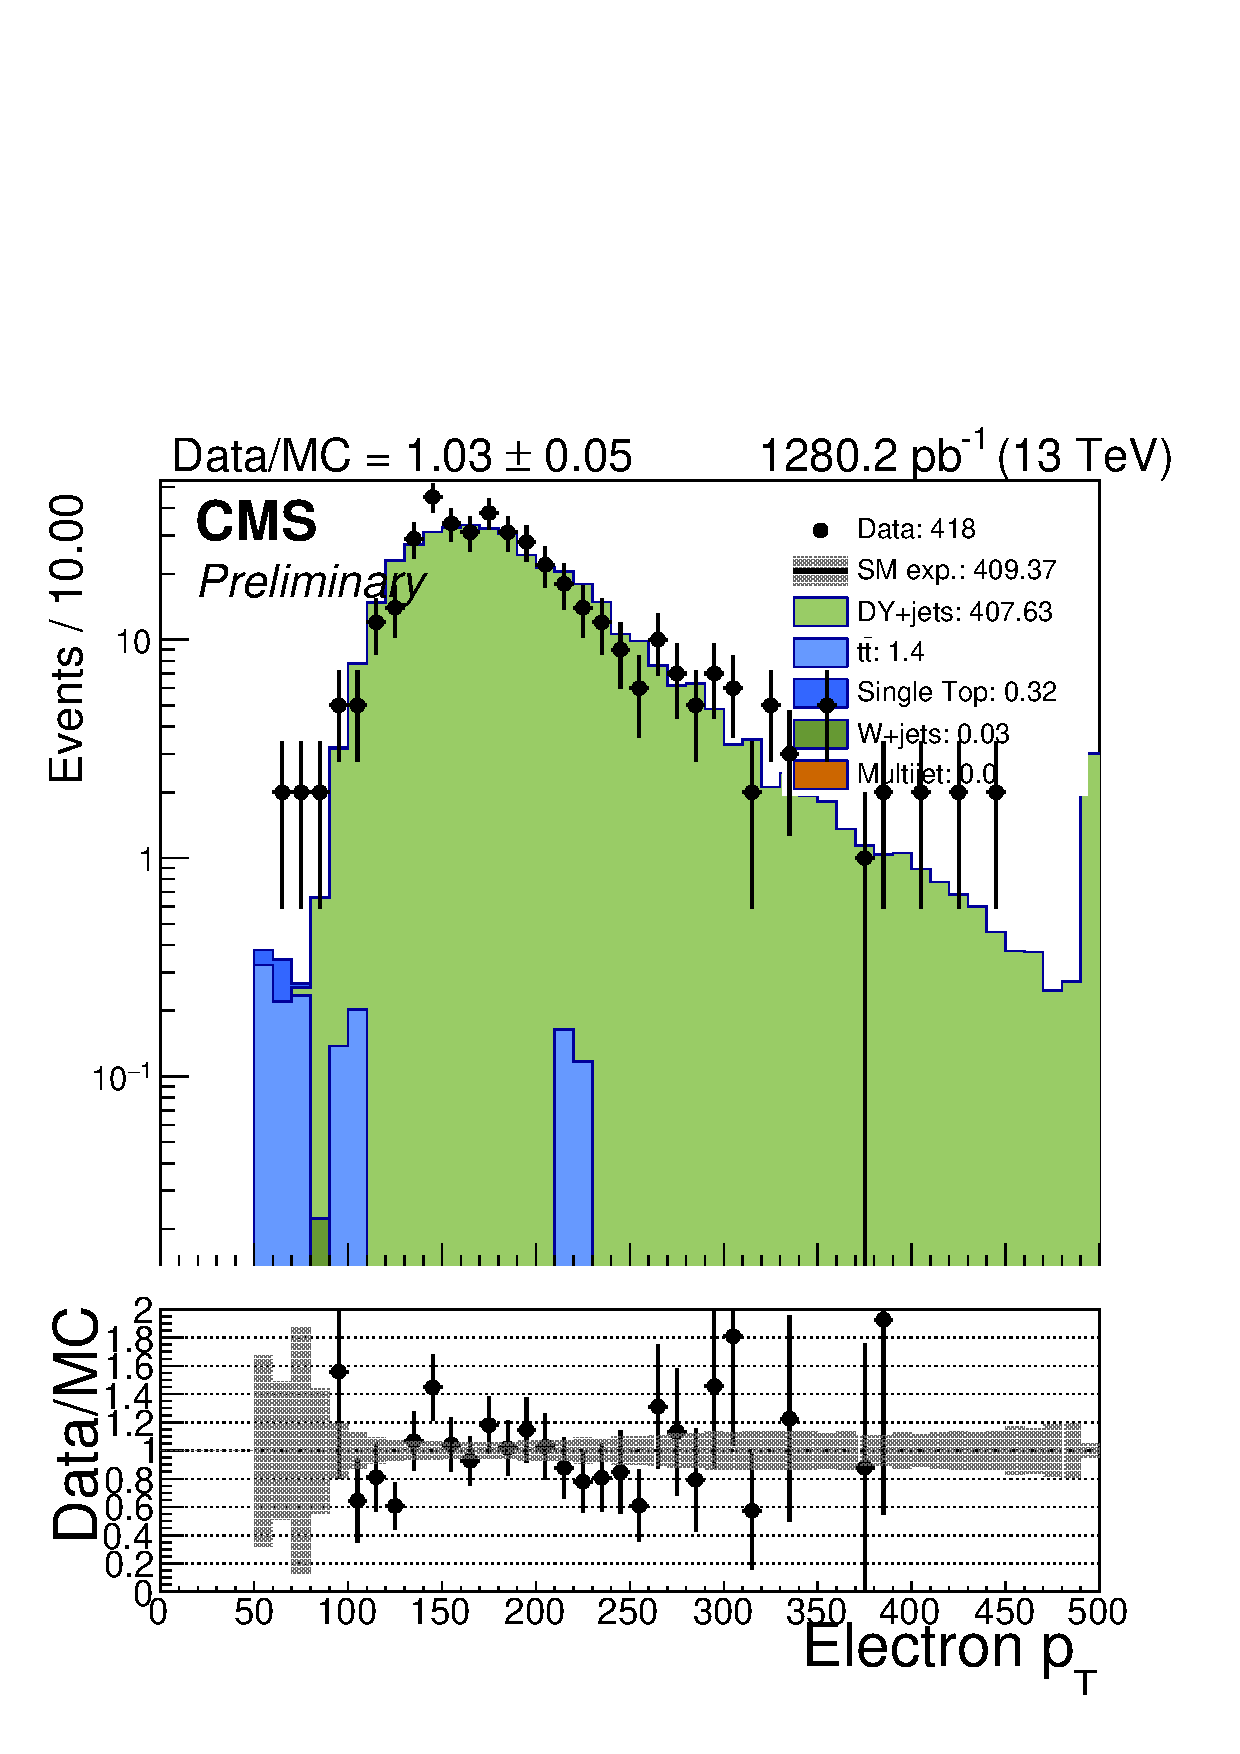
\includegraphics[width=0.5\textwidth]{figures/distributions/DoubleEle/ele_pt[0]_eq1j.pdf}} \\
%        \caption{Key analysis variables for double electron control region (monojet bins)}
%        \label{fig:distribution_doubleele_mono}
%    \end{center}
%\end{figure}


